\documentclass[dvips,landscape]{foils}
\usepackage{graphicx,psfrag}
\usepackage{graphics}
\usepackage{amsmath}
\usepackage{amsthm}
\usepackage{amsfonts}
\input defs.tex
\raggedright
\special{! TeXDict begin /landplus90{true}store end }
\renewcommand{\oursection}[1]{
\foilhead[-1.0cm]{#1}
}

\title{The Mixing Property of Chaotic Maps and Cutoff Phenomenon}
\author{Tzu-Chen Liang}
\MyLogo{Tzu-Chen Liang, Stanford University}
\date{\today}
\newtheorem{definition}{Definition}
\newtheorem{example}{Example}
\newtheorem{theorem}{Theorem}
\newtheorem{lemma}{Lemma}

\begin{document}
%\setlength{\parskip}{0cm}
\maketitle


%%%%%%%%%%%%%%%%%%%%%%%%%%%%%%%%%%%%%%%%%%%%%%%%%%%%%%%%%%%%%%%%%%%%%%%%
\newpage
\oursection{Riffle Shuffle Problem}
\begin{itemize}
\item Question: How many shuffles are necessary and sufficient to approximately randomize $52$ cards?
\end{itemize}
\centerline{
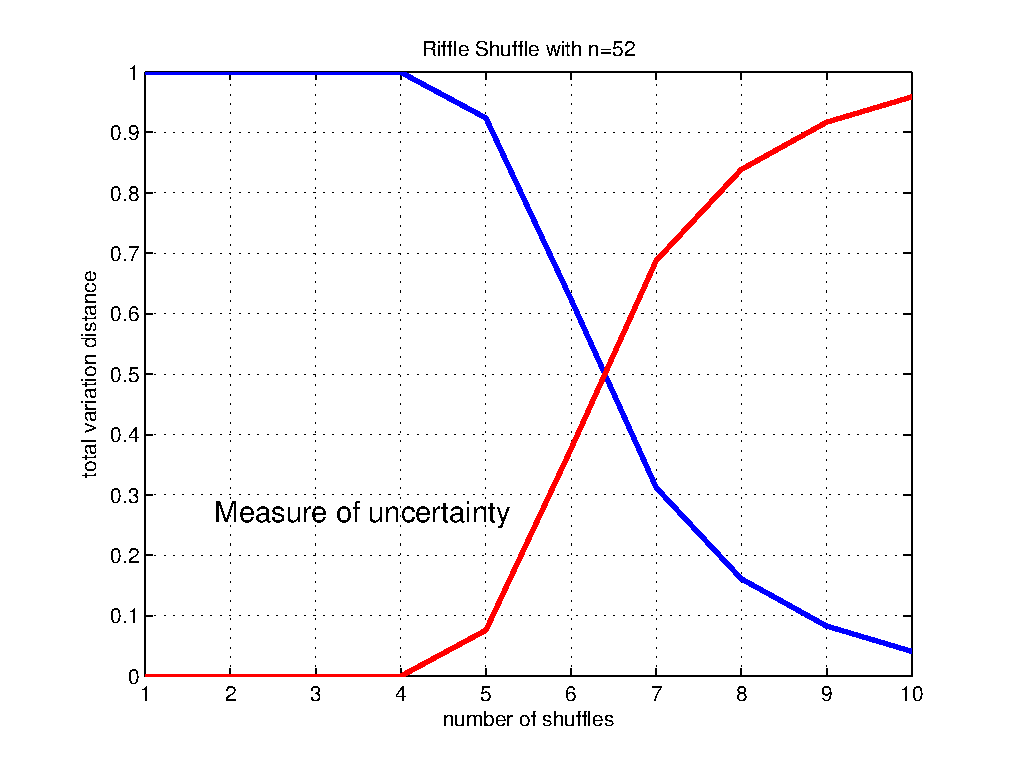
\includegraphics[width=0.50\textwidth,trim=1cm 1cm 0cm 0cm]{riffleshuffle2}
}

%%%%%%%%%%%%%%%%%%%%%%%%%%%%%%%%%%%%%%%%%%%%%%%%%%%%%%%%%%%%%%%%%%%%%%%%%
\newpage
\oursection{Motivation}
\begin{itemize}
\item How does the measure of uncertainty evolve when a probability distribution is transported by a chaotic map?
\item How does a chaotic map mix scalar functions?
\end{itemize}
{\bfseries Goal}
\begin{itemize}
\item Relate the above two questions to cutoff phenomenon in finite Markov chains.
\item Show evidence of cutoff in chaotic map simulations. 
\end{itemize}

%%%%%%%%%%%%%%%%%%%%%%%%%%%%%%%%%%%%%%%%%%%%%%%%%%%%%%%%%%%%%%%%%%%%%%%%%
\newpage
\oursection{Cutoff Phenomenon}

\begin{example} \textbf{Random walk on an $n$-dimensional hypercube}
a particle starts at $\mathbf{0}$ and moves to one of its nearest neighbors (or stay fixed) with equal probability at each step.

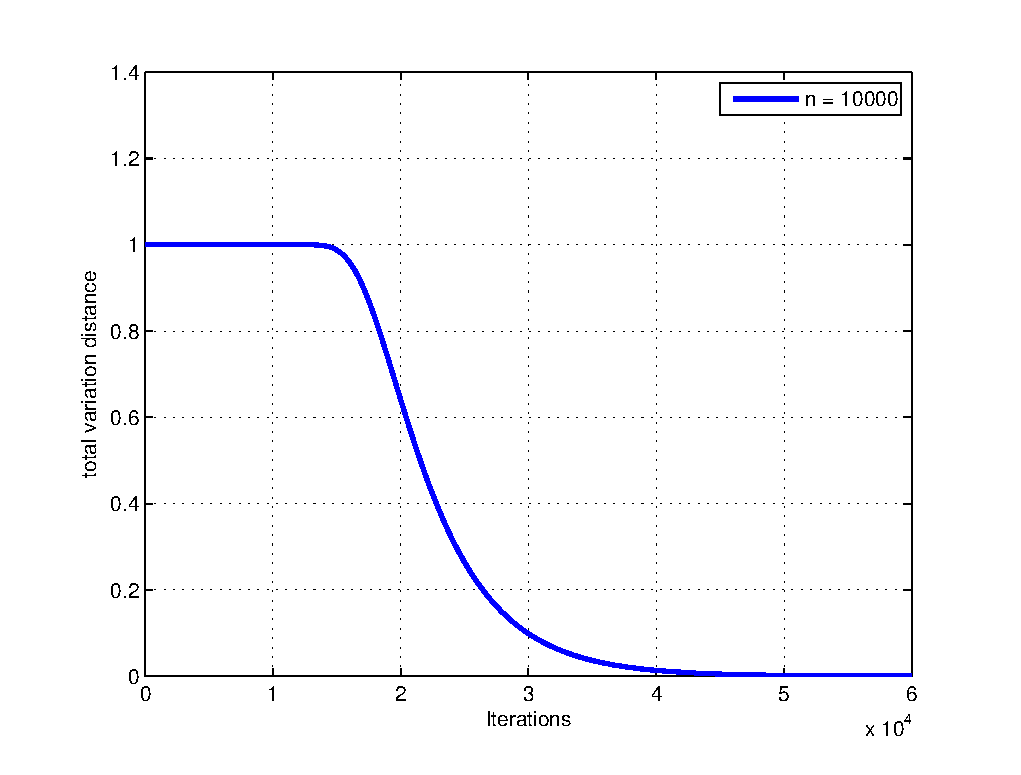
\includegraphics[width=0.45\textwidth,trim=1cm -1cm 0cm 0cm]{cutoffexample}
\parbox[b]{12cm}{
  Total Variation Distance
  \begin{eqnarray*}
   \|\omega^k - \bar{\omega}\|_{TV} &=& \frac{1}{2}\sum_{i=1}^n |\omega_i^k-\bar{\omega}_i |\\
               &=& \frac{1}{2}\sum_{i=1}^n |f_i^k-1|\bar{\omega}_i
  \end{eqnarray*}
  where $f^k_i = \omega_i^k/\bar{\omega}_i$. $f$ is the density of $\omega$ with respect to $\bar{\omega}$.
   }
    $\omega^k$: state distribution at time $k$, 
    $\bar{\omega}$: invariant distribution  
\end{example} 

%%%%%%%%%%%%%%%%%%%%%%%%%%%%%%%%%%%%%%%%%%%%%%%%%%%%%%%%%%%%%%%%%%%%%%%%%
\newpage
Assume that, to any finite set $\Omega$ and any
pair of probability measures $\omega$, $\nu$ on $\Omega$ is associated
a real number $D(\omega,\nu)$ such that $D(\omega,\nu)\in [0,1]$,

\begin{eqnarray}
\max_{\Omega,\omega,\nu} D(\omega,\nu) = 1
\end{eqnarray}
and $D(\omega,\nu)=0$ if and only if $\omega=\nu$. Consider a sequence of
(finite) probability spaces $(\Omega_n,\nu_n)$, $n=1,2,...$, each
equipped with a sequence of probability measure $\omega^k_n$,
$l=0,1,...$, such that
\begin{eqnarray}
\lim_{k \rightarrow \infty} D(\omega^k_n,\nu_n)=0
\end{eqnarray}
%%%%%%%%%%%%%%%%%%%%%%%%%%%%%%%%%%%%%%%%%%%%%%%%%%%%%%%%%%%%%%%%%%%%%%%%%
\newpage
\begin{definition}
\label{cutoffdefition}
(Diaconis) A family $(\Omega_n,\nu_n, (\omega^k_n)_{k=0,1,...})_{n=1,2,...}$
presents a D-cut-off if there exists a sequence $(t_n)$ of positive
reals such that, for any $\epsilon \in(0,1)$,
\begin{enumerate} \setlength{\parskip}{0pt}  \setlength{\itemsep}{-0pt} \setlength{\topsep}{0pt} %\setlength{\parsep}{70pt}% 
  \item $\lim_{k \rightarrow \infty}D(\omega^{k_n}_n,\nu_n) = 0 \mbox{ if }
  k_n>(1+\epsilon)t_n$
  \item $\lim_{k \rightarrow \infty}D(\omega^{k_n}_n,\nu_n) = 1 \mbox{ if }
  k_n<(1-\epsilon)t_n $
\end{enumerate}
\end{definition}
\centerline{
\begin{tabular}{rl}%\setlength{\tabcolsep}{-30mm}
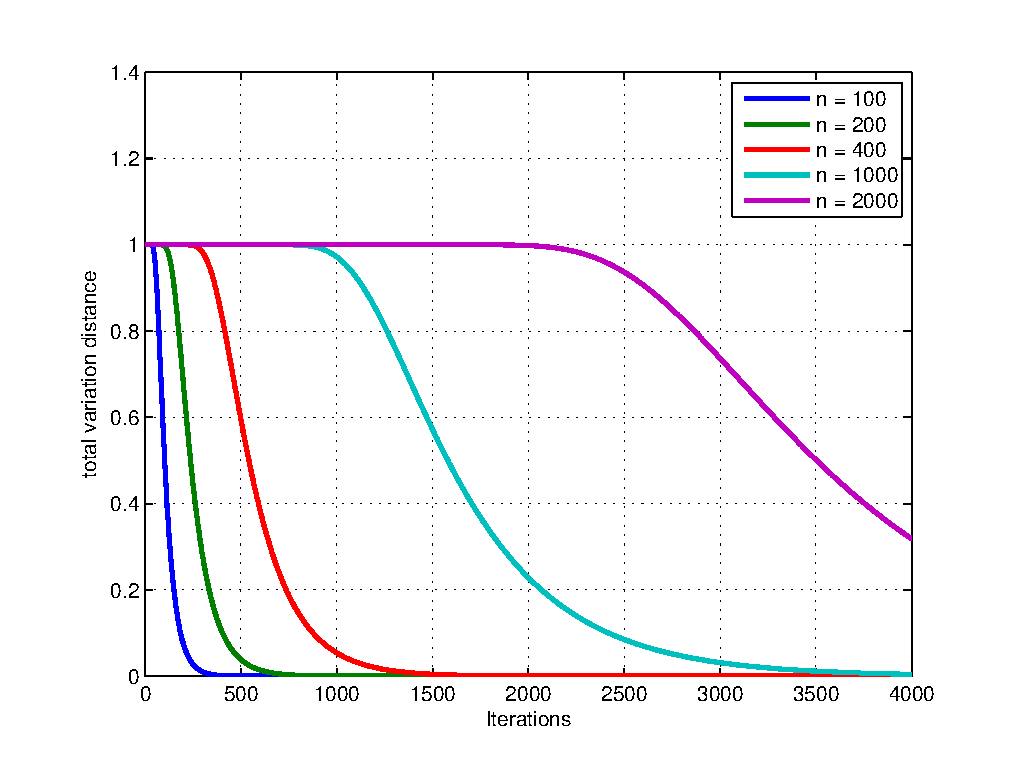
\includegraphics[width=0.43\textwidth,trim=1cm 1cm 0cm 0cm]{rdwalk}&
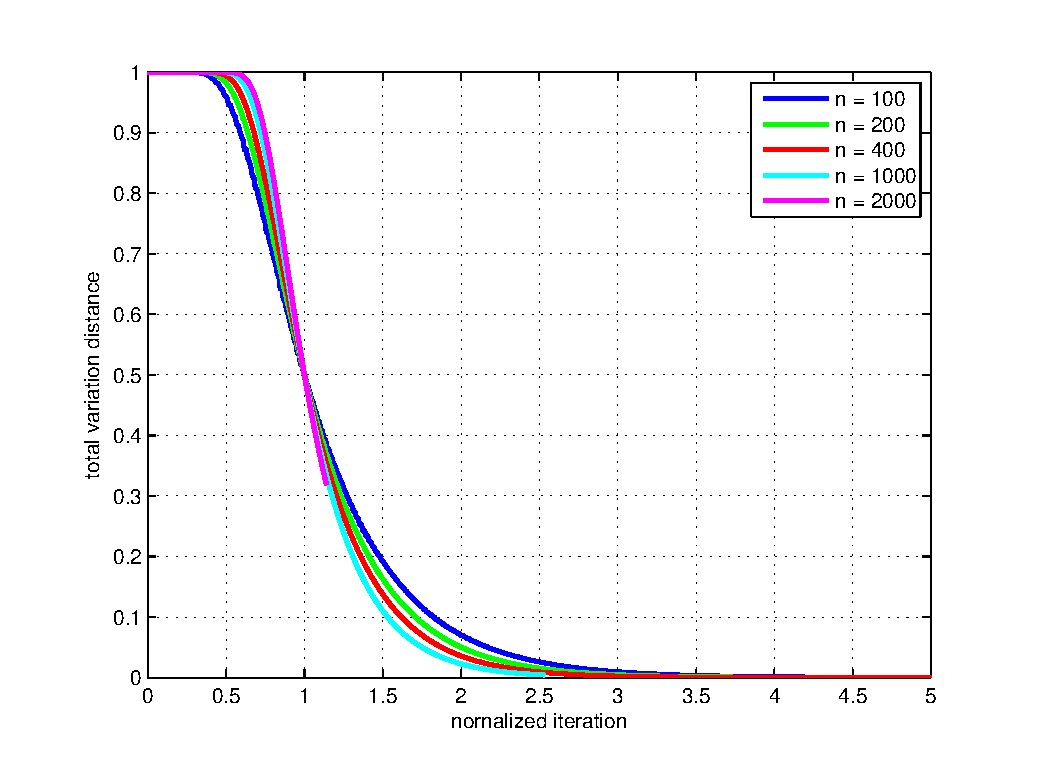
\includegraphics[width=0.43\textwidth,trim=1cm 1cm 0cm 0cm]{rdwalkn}
\end{tabular}
}

%%%%%%%%%%%%%%%%%%%%%%%%%%%%%%%%%%%%%%%%%%%%%%%%%%%%%%%%%%%%%%%%%%%%%%%%%
\newpage
\oursection{Cutoff Phenomenon}
\begin{itemize}
\item The behavior of a sequence of Markov chain.
\item Depends on the distance function $D$.
\item Depends on the initial distribution.
\item Usually observed in large systems.
\end{itemize}

Let us relax the definition: $\Omega_n$ can be infinite 
%%%%%%%%%%%%%%%%%%%%%%%%%%%%%%%%%%%%%%%%%%%%%%%%%%%%%%%%%%%%%%%%%%%%%%%%%
\newpage
\oursection{Tent Map and Logistic Map}

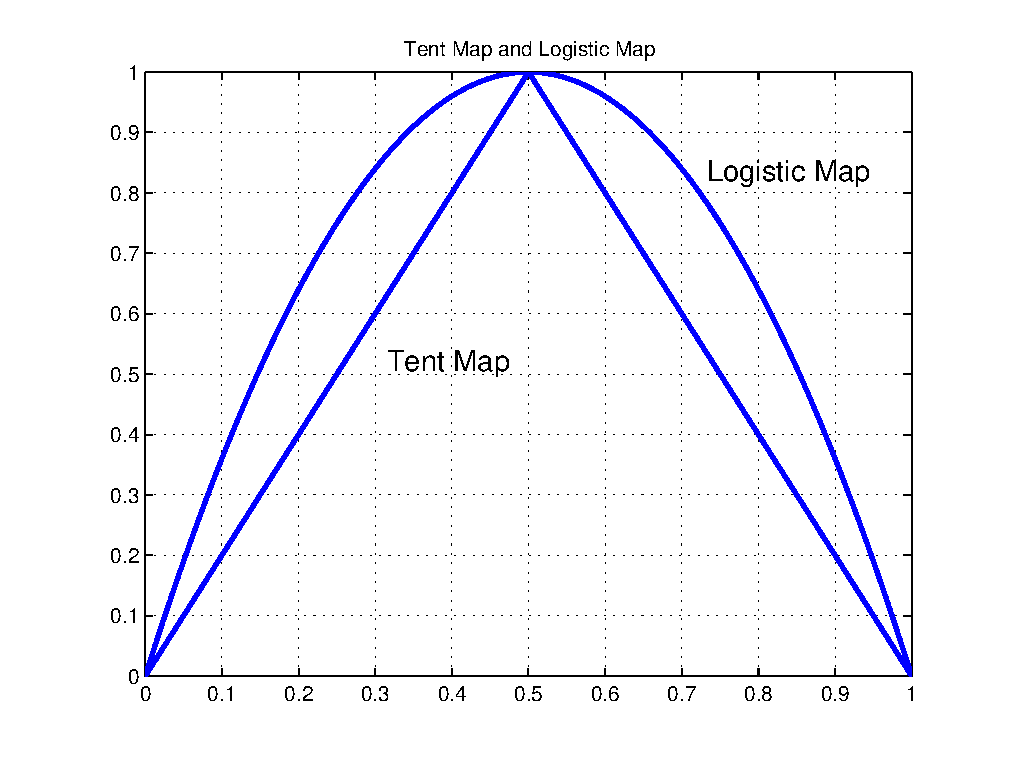
\includegraphics[width=0.42\textwidth,trim=1cm 1cm 0cm 0cm]{tentmapandlogisticmap}
\parbox[b]{12cm}{
\begin{itemize}
\item Tent Map
  \begin{eqnarray}
    x' = 1-2\left|x-\frac{1}{2}\right| 
  \end{eqnarray}
\item Logistic Map ($r=4$)
  \begin{eqnarray}
    x' = rx(1-x) 
  \end{eqnarray}
\end{itemize}
}

Both maps are known to be chaotic. They are equivalent via a transformation. 
%%%%%%%%%%%%%%%%%%%%%%%%%%%%%%%%%%%%%%%%%%%%%%%%%%%%%%%%%%%%%%%%%%%%%%%%%%
\newpage
\oursection{Probability Distribution Evolved by a Map}
For a given 1-D map $S:x \mapsto x' $. The probability measure $\omega(x),x \in [0,1]$ transported by $S$ in the following way, 
  \begin{eqnarray}
    \omega'(x')|dx'| = \omega(x)|dx|
  \end{eqnarray}
It is possible that there are more than one $x$ which give the same $x'$. Hence we actually have,
  \begin{eqnarray}
  \label{omegamap}
    \omega'(x') = \sum_i \left|\frac{dx_i}{dx'}\right|\omega(x) \mbox{   , for all } i \mbox{  such that  } x'=S(x_i)
  \end{eqnarray}
%%%%%%%%%%%%%%%%%%%%%%%%%%%%%%%%%%%%%%%%%%%%%%%%%%%%%%%%%%%%%%%%%%%%%%%%%%
\newpage
\oursection{Tent Map Cutoff}
with the following initial distribution on $[0 ,1]$
  \begin{eqnarray}
  \label{tentmapinitial}
    \omega_{\mu_n}^0 = \left\{ \begin{tabular}{c}
                      $\frac{1}{\mu_n}$, \mbox{  if  } $x \le \mu_n$\\ 
                      $0$, \mbox{  otherwise} 
                      \end{tabular}\right.
  \end{eqnarray}
where $\mu_1 = 1$, and $\mu_{n+1} = \frac{\mu_n}{2}$. By applying (\ref{omegamap}), we have
  \begin{eqnarray}
  \label{tentmapevolve}
    \omega_{\mu_n}^{k+1}(x) = \frac{1}{2}\left( \omega_{\mu_n}^{k}\left(\frac{x}{2}\right)+
                                                \omega_{\mu_n}^{k}\left(1-\frac{x}{2}\right)  \right)
  \end{eqnarray}
The invariant distribution $\bar{\omega}$ of tent map is uniform. Now consider the following sequence,
 \begin{eqnarray}
  \nu_{\mu_n}^k \equiv  \frac{1}{2}|\omega_{\mu_n}^k-\bar{\omega} | 
 \end{eqnarray}
%%%%%%%%%%%%%%%%%%%%%%%%%%%%%%%%%%%%%%%%%%%%%%%%%%%%%%%%%%%%%%%%%%%%%%%%%%
\newpage
 \begin{eqnarray}
   \nu_{\mu_n}^k =  \left\{ \begin{tabular}{c} 
                    $1- 2^{1+k-n} $  ,if $k \le n-1$ \\
                    $0$   , otherwise
                    \end{tabular}\right.
 \end{eqnarray}
\centerline{
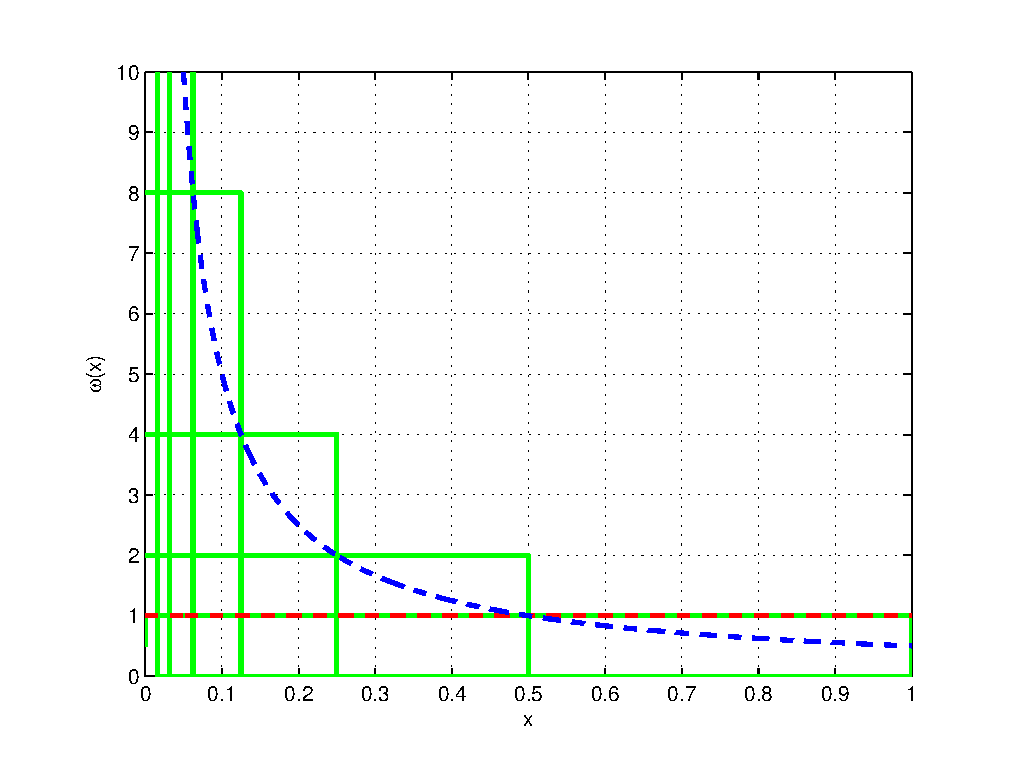
\includegraphics[width=0.48\textwidth,trim=1cm 1cm 0cm 0cm]{tentmapsimu.eps}
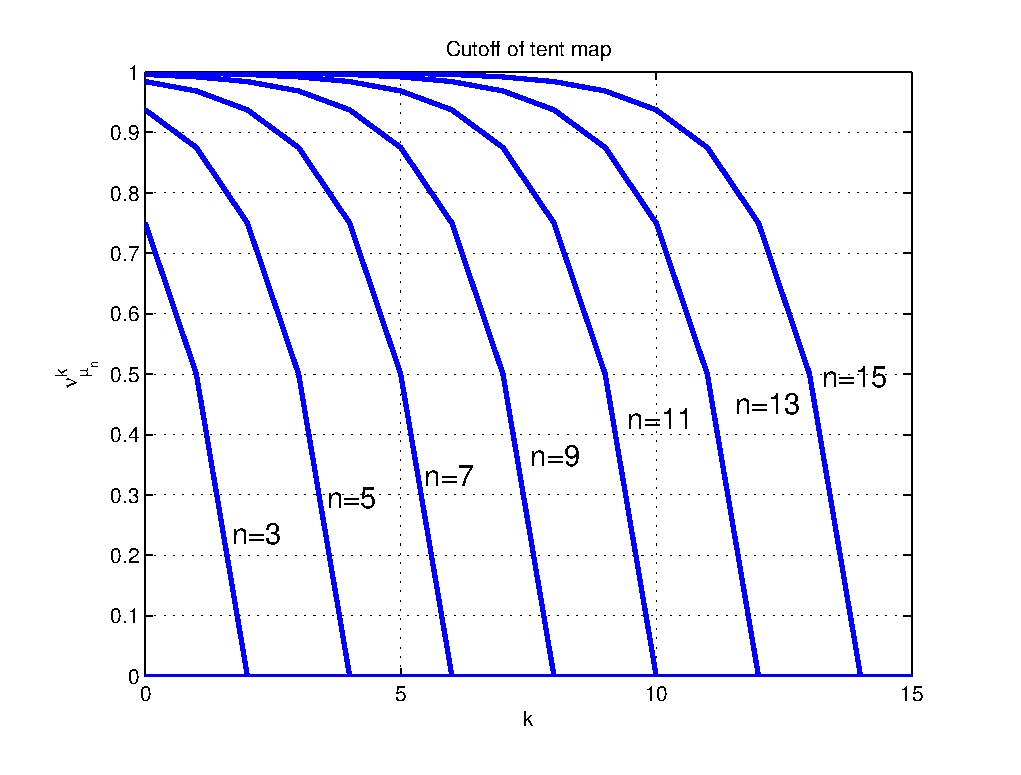
\includegraphics[width=0.48\textwidth,trim=1cm 1cm 0cm 0cm]{tentmapcutoff.eps}
}
%%%%%%%%%%%%%%%%%%%%%%%%%%%%%%%%%%%%%%%%%%%%%%%%%%%%%%%%%%%%%%%%%%%%%%%%%%
\newpage
\centerline{
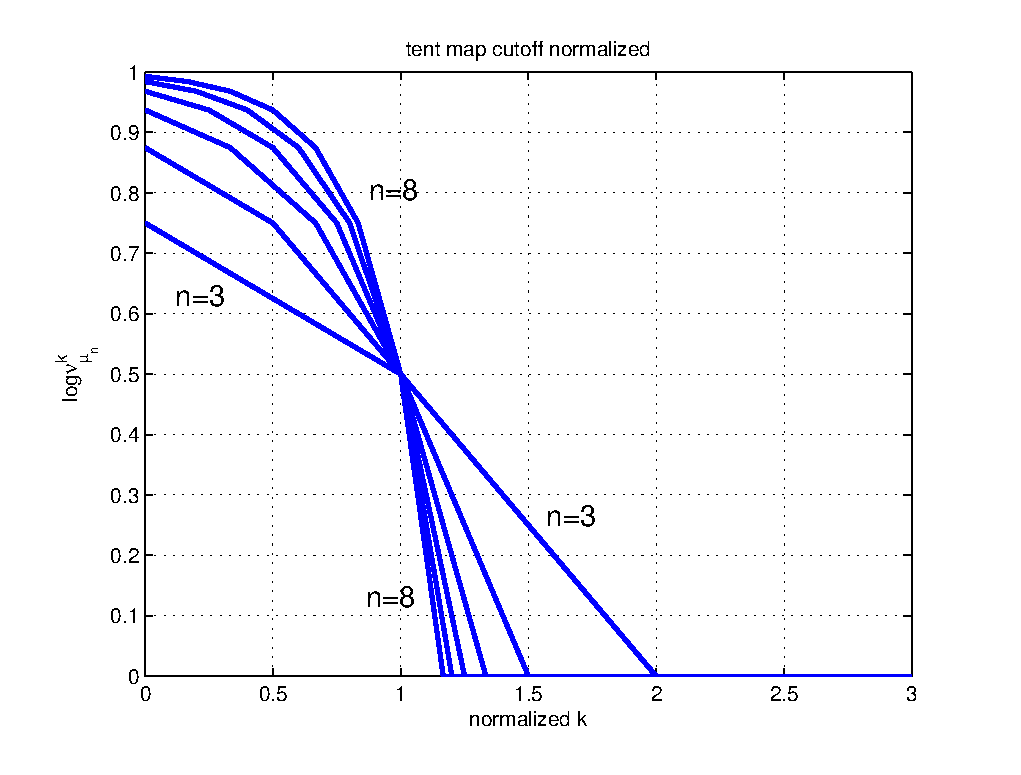
\includegraphics[width=0.48\textwidth,trim=0cm 0cm 0cm 0cm]{tentmapcutoffnormalized.eps}
}
\begin{theorem} {\bfseries (Tent map cutoff)}

The family $([0,1],\bar{\omega}, (\omega^k_{\mu_n})_{k=0,1,...})_{n=1,2,...}$, where $\bar{\omega}$ is uniform in $[0,1]$ and $\omega^k_{\mu_n}$ are defined as in (\ref{tentmapinitial}) and (\ref{tentmapevolve}), presents a Total Variation-cut-off in the relaxed sense.
\end{theorem}


%%%%%%%%%%%%%%%%%%%%%%%%%%%%%%%%%%%%%%%%%%%%%%%%%%%%%%%%%%%%%%%%%%%%%%%%%%
\newpage
\oursection{Logistic Map Cutoff}


with $r = 4$. Define initial distributions as
  \begin{eqnarray}
  \label{omegamun0}
  \label{logisticmapinitial}
    \omega_{\mu_n}^0 = \left\{ \begin{tabular}{c}
                      $\frac{1}{\mu_n}$, \mbox{  if  } $x \le \mu_n$\\ 
                      $0$, \mbox{  otherwise} 
                      \end{tabular}\right.
  \end{eqnarray}
but now with  $\mu_0=1$, $\mu_{n+1}=\frac{1-\sqrt{1-\mu_n}}{2}$.

Again, by applying (\ref{omegamap}), we have
 \begin{eqnarray}
 \label{logisticmapevolve}
    \omega_{\mu_n}^{k+1}(x) = \frac{1}{4\sqrt{1-x}}\left( \omega_{\mu_n}^{k}\left( \frac{1-\sqrt{1-x}}{2}\right)
                                            +\omega_{\mu_n}^{k}\left( \frac{1+\sqrt{1-x}}{2}\right) \right)
 \end{eqnarray}
%%%%%%%%%%%%%%%%%%%%%%%%%%%%%%%%%%%%%%%%%%%%%%%%%%%%%%%%%%%%%%%%%%%%%%%%%%
\newpage

The invariant distribution $\bar{\omega}$ for logistic map is 
\begin{eqnarray} 
\label{logisticmapinvariant}
 \bar{\omega} = \frac{1}{\pi\sqrt{x(1-x)}}
\end{eqnarray}

\centerline{
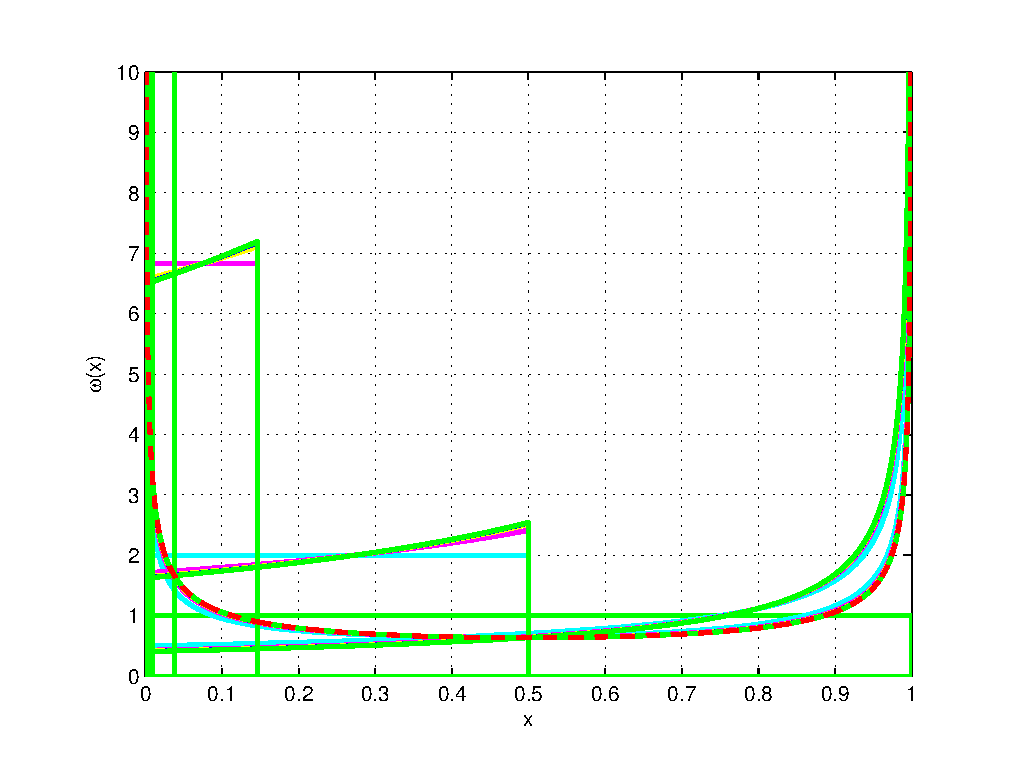
\includegraphics[width=0.59\textwidth,trim=1cm 1cm 0cm 0cm]{logisticmapsimu.eps}
}
%%%%%%%%%%%%%%%%%%%%%%%%%%%%%%%%%%%%%%%%%%%%%%%%%%%%%%%%%%%%%%%%%%%%%%%%%%
\newpage

\centerline{
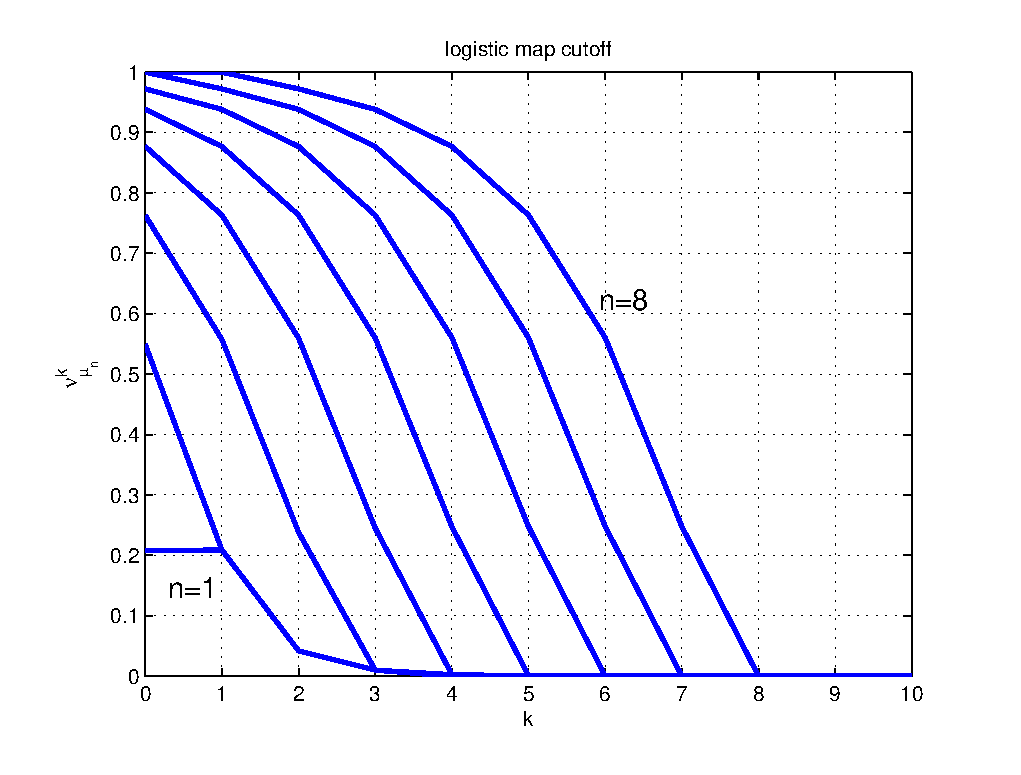
\includegraphics[width=0.50\textwidth,trim=0cm 0cm 0cm 0cm]{logisticmapcutoff.eps}
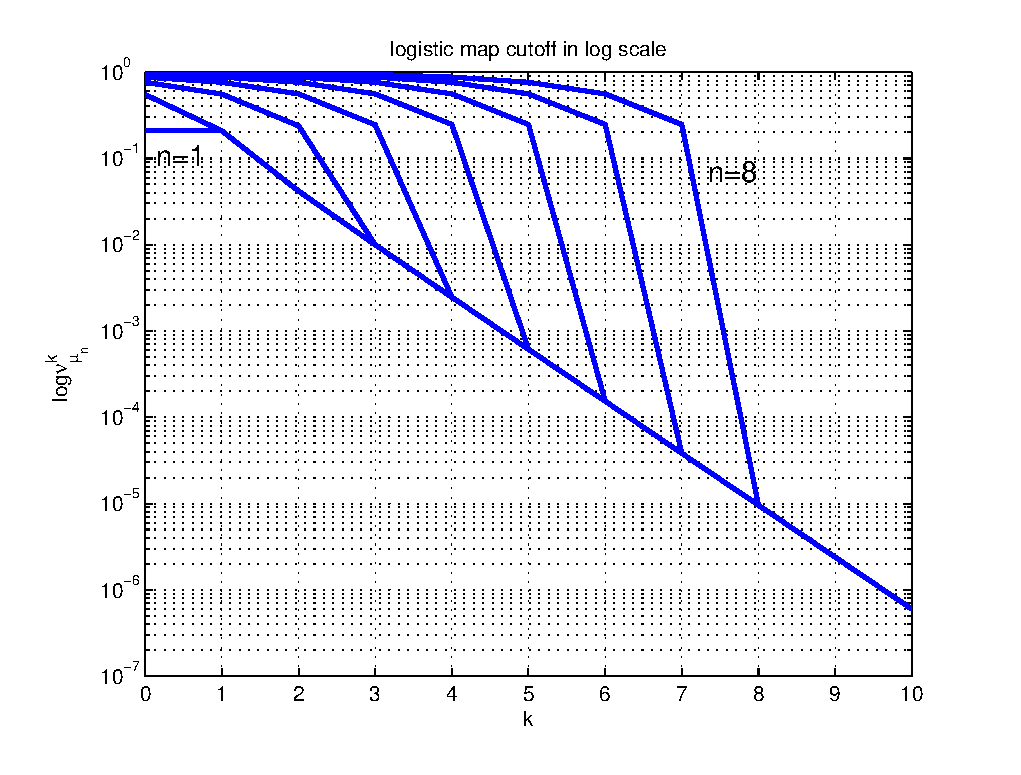
\includegraphics[width=0.50\textwidth,trim=0cm 0cm 0cm 0cm]{logisticmapcutofflog.eps}
}
\begin{lemma} For all $k \le n$,
$$|\omega_{\mu_n}^k - \bar{\omega}|_{TV}>|\omega_{\mu_n-1}^{k-1} - \bar{\omega}|_{TV}$$
\end{lemma}


\begin{lemma}For all $k \ge n$,
$$\omega_{\mu_n}^k = \omega_{\mu_{n-1}}^{k}$$
\end{lemma}
%%%%%%%%%%%%%%%%%%%%%%%%%%%%%%%%%%%%%%%%%%%%%%%%%%%%%%%%%%%%%%%%%%%%%%%%%%
\newpage
\centerline{
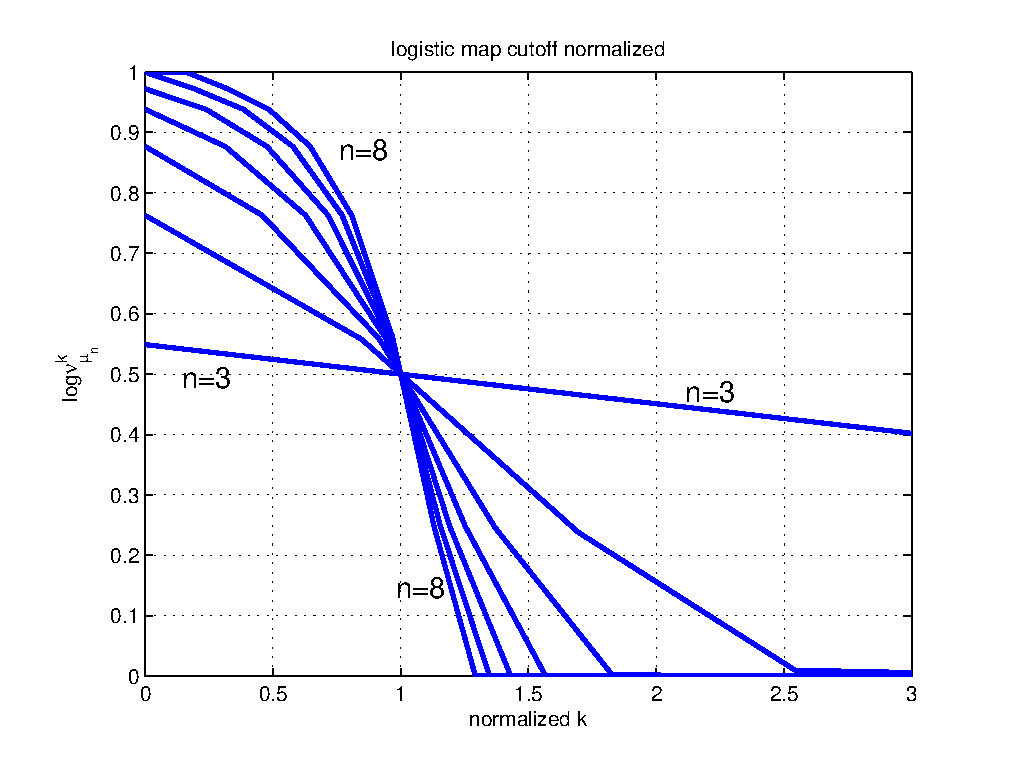
\includegraphics[width=0.48\textwidth,trim=0cm 0cm 0cm 0cm]{logisticmapcutoffnormalized.eps}
}
\begin{theorem} {\bfseries (Logistic map cutoff)}

The family $([0,1],\bar{\omega}, (\omega^k_{\mu_n})_{k=0,1,...})_{n=1,2,...}$, where $\bar{\omega}$ is defined as in (\ref{logisticmapinvariant}) and $\omega^k_{\mu_n}$ are defined as in (\ref{logisticmapinitial}) and (\ref{logisticmapevolve}), presents a Total Variation-cut-off between $k=n-1$ and $n$ in the relaxed sense .
\end{theorem}
%%%%%%%%%%%%%%%%%%%%%%%%%%%%%%%%%%%%%%%%%%%%%%%%%%%%%%%%%%%%%%%%%%%%%%%%%%
\newpage
\oursection{Another Map}
 \begin{eqnarray}
    x' = \sin(\pi x)
 \end{eqnarray}
\centerline{
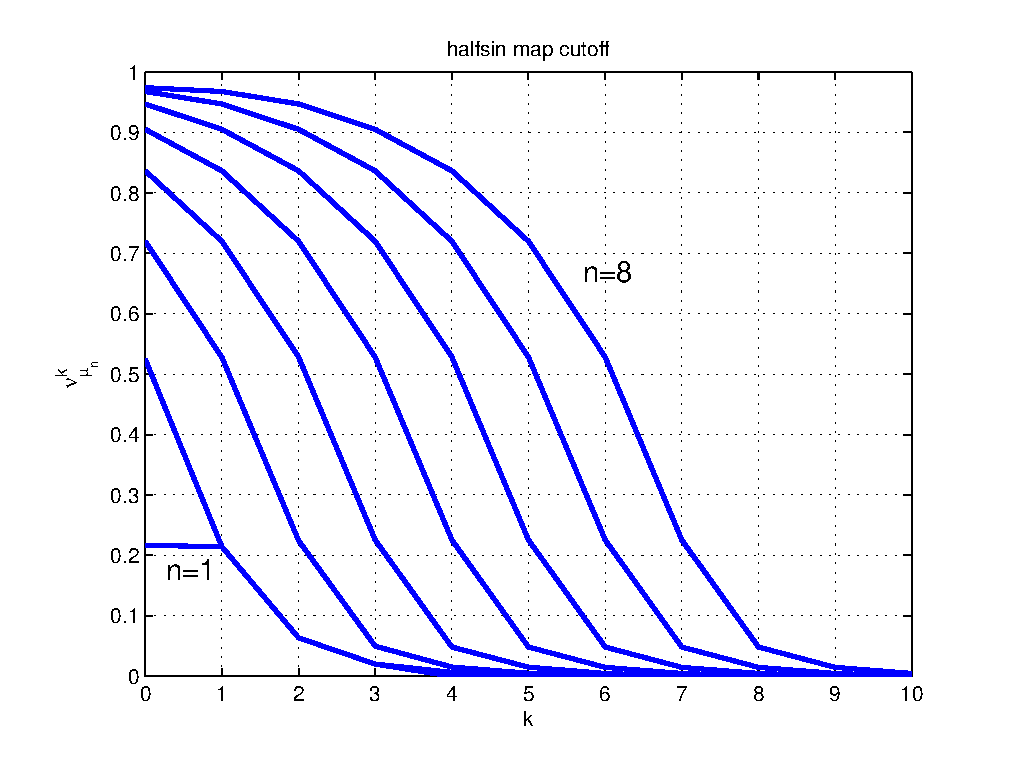
\includegraphics[width=0.50\textwidth,trim=1cm 1cm 0cm 0cm]{halfsinmapcutoff.eps}
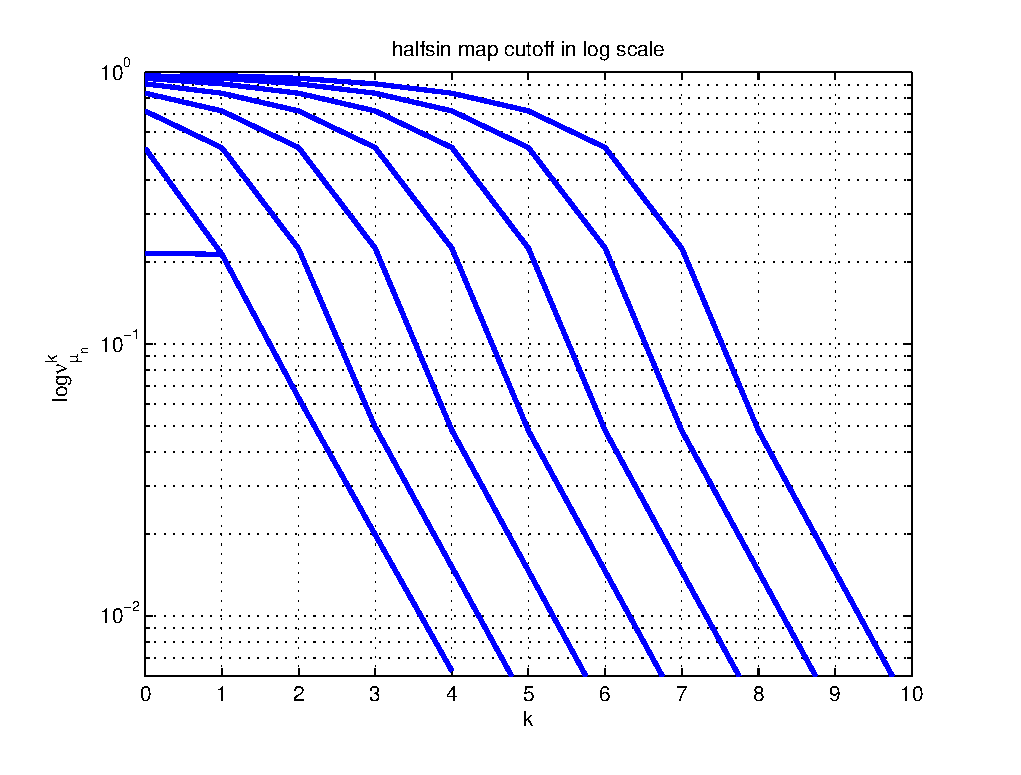
\includegraphics[width=0.50\textwidth,trim=1cm 1cm 0cm 0cm]{halfsinmapcutofflog.eps}
}
Still it presents a cutoff, but hard to prove.


%%%%%%%%%%%%%%%%%%%%%%%%%%%%%%%%%%%%%%%%%%%%%%%%%%%%%%%%%%%%%%%%%%%%%%%%%
\newpage
\oursection{A Chart}
\renewcommand{\arraystretch}{1.3}
\begin{tabular}{l|cc}

                      & We have done                    & We are going to do     \\
\hline
        Method        & Analytical                      & Numerical    \\
\hline
        Operator      & the same map, eq(6)                  & $A_n$, $\lim_{n \rightarrow \infty} A_n = A$ \\
\hline
        IC            &  $\omega_{\mu_n}^0 = \left\{ \begin{array}{c}
                                     \frac{1}{\mu_n}, \mbox{  if  } x \le \mu_n\\ 
                      0, \mbox{  otherwise} 
                      \end{array}\right.$
                                                          & $f^0 = g_n(\cos(2 \pi x))$ \\
\hline
$\nu^k$               &  $\frac{1}{2}\int_X |f^k-1|\bar{\omega}dx$,$f^k= \frac{\omega^k}{\bar{\omega}}$
                    
                                                        &   $\frac{1}{2}\sum_{i=1}^n |f^k_i-1|$

  
\end{tabular}

where $g_n: X \rightarrow \mathbb{R}^n$, for the grid $a_i$,
\begin{eqnarray}
  g_n(f(\mathbf{x}))_i = \int_{a_i} f(\mathbf{x}) d\mathbf{x}
\end{eqnarray}

%%%%%%%%%%%%%%%%%%%%%%%%%%%%%%%%%%%%%%%%%%%%%%%%%%%%%%%%%%%%%%%%%%%%%%%%%%
\newpage
\oursection{The Mixing Property of Chaotic Maps with Small Diffusion}
\begin{itemize}
\item The decay of the variance of a passive scalar function in a chaotic flow with diffusion
\item Add a smoothing(diffusion) step between each transformation -- Advection-Diffusion operator.
\item Multi-stage transition has been found in many cases. 
\item Hard to simulate numerically. 
\item No agreement about what will happen in the zero-diffusion limit.
\end{itemize}
%%%%%%%%%%%%%%%%%%%%%%%%%%%%%%%%%%%%%%%%%%%%%%%%%%%%%%%%%%%%%%%%%%%%%%%%%%
\newpage
{\bfseries"Chaotic Mixing in a Torus Map", Jean-Luc Thiffeault, June , 2006}
Modified Arnold's cat map with small diffusion
\centerline{
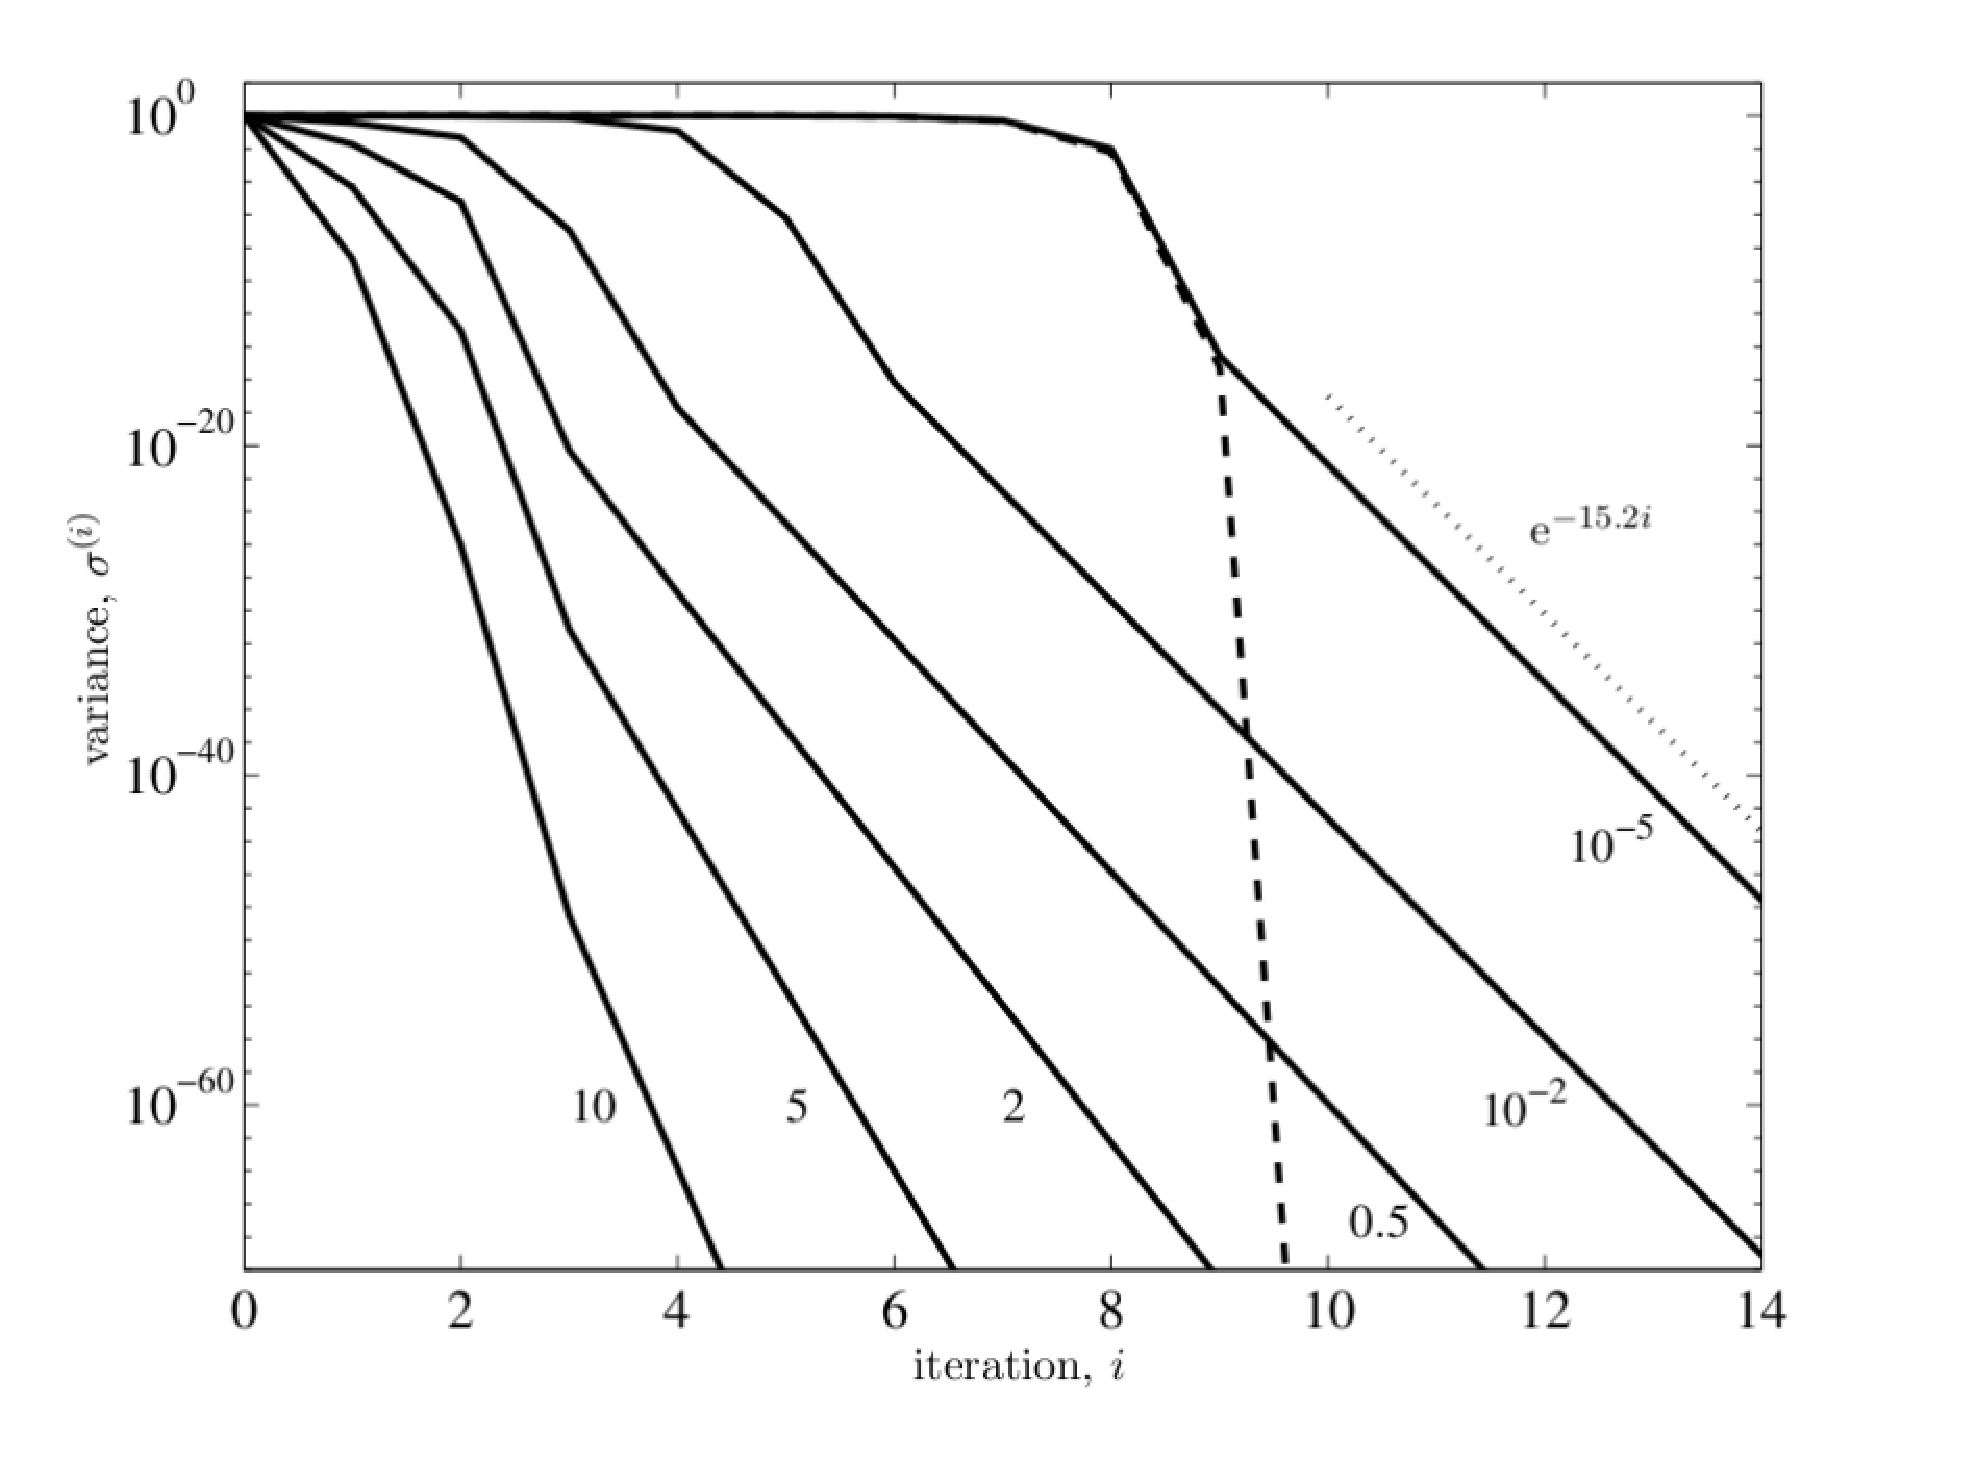
\includegraphics[width=0.6\textwidth,trim=1cm 1cm 0cm 0cm]{catmap}
}
Decay of total variance for varying diffusivity from $10$ to $1e-5$



\newpage
\centerline{
\begin{tabular}{rl}%\setlength{\tabcolsep}{-30mm}
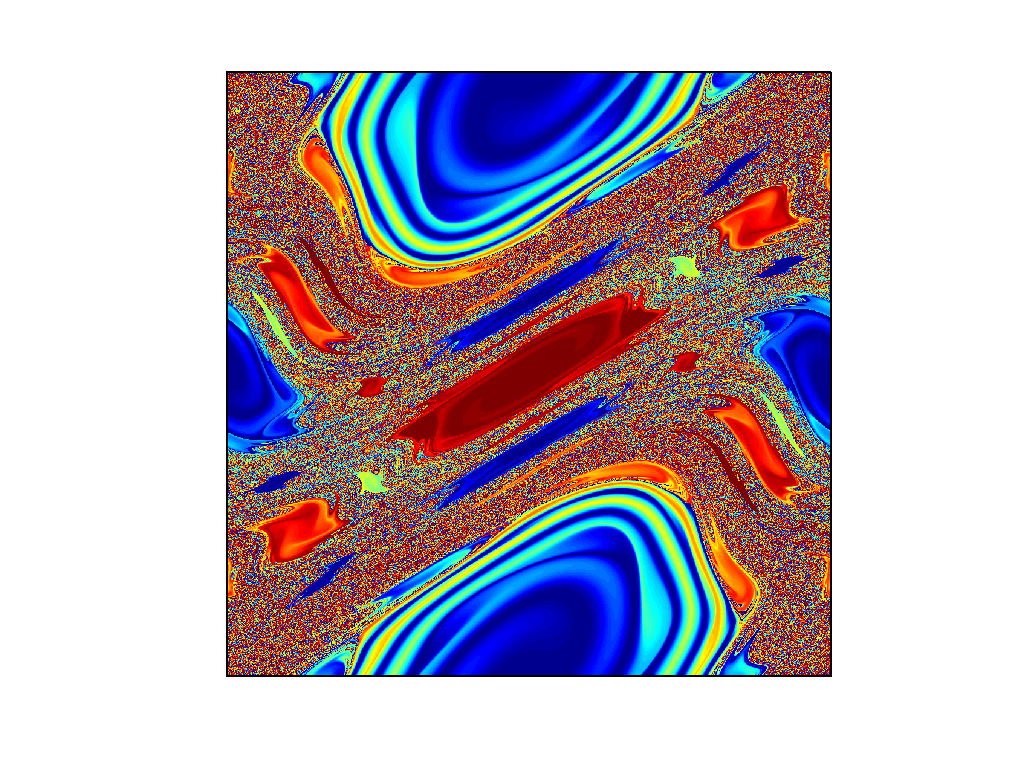
\includegraphics[width=0.55\textwidth,trim=1cm 1cm 0cm 0cm]{standardmapsimuexact}&
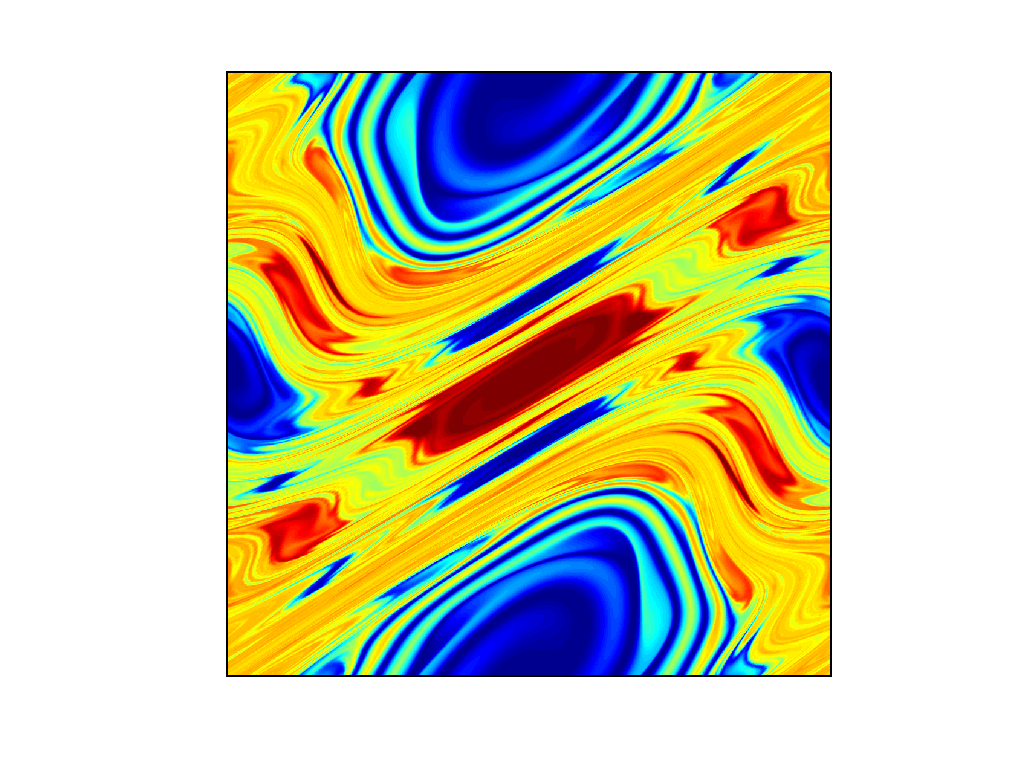
\includegraphics[width=0.55\textwidth,trim=1cm 1cm 0cm 0cm]{standardmapsimumarkov}
\end{tabular}
}
\begin{itemize}
\item Simulation of Standard map. (Left figure)
\item Simulation of Standard map with small diffusion. (Right figure)
%\item Left figure is done by advecting the grid points backward 40 times and finding its color at $k=0$
%\item Right figure is the Markov chain simulation.  
\end{itemize}
%%%%%%%%%%%%%%%%%%%%%%%%%%%%%%%%%%%%%%%%%%%%%%%%%%%%%%%%%%%%%%%%%%%%%%%%%%
\newpage
\oursection{Degree of Chaos: Ergodic, Mixing and Exact}
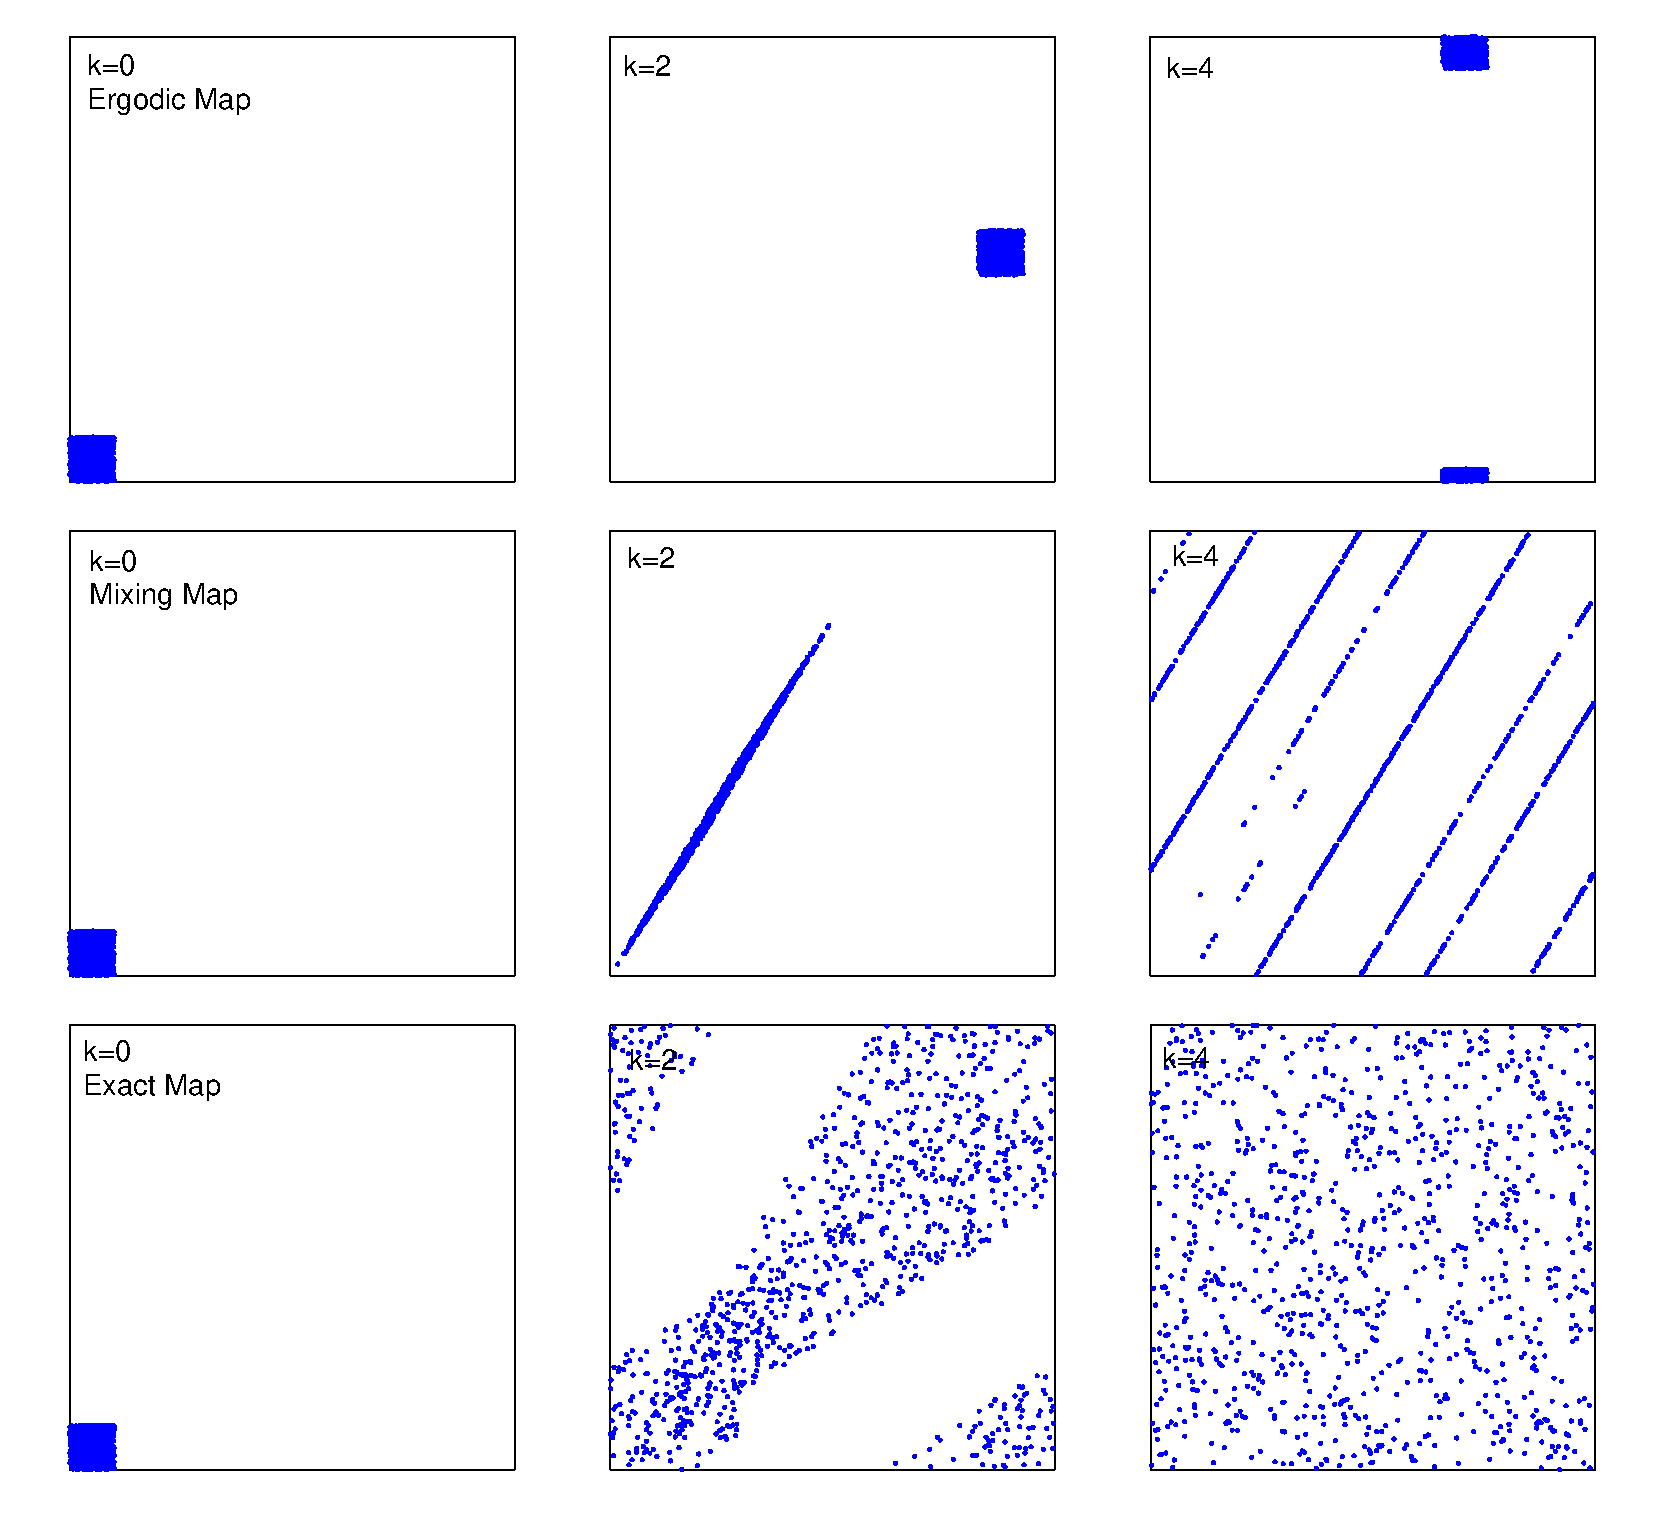
\includegraphics[width=0.5\textwidth,trim=1cm 1cm 1cm 1cm]{ergodicmixingandexact}
\parbox[b]{10cm}{
\begin{itemize}
\setlength{\topsep}{0cm}
\setlength{\parskip}{0cm}
\setlength{\parsep}{0.5cm}
\setlength{\itemsep}{1.2cm}
\item {\bfseries (Ergodic)} If every invariant set $A\in \mathcal{A}$ is such that $\mu(A)=0$ or $\mu(X \setminus A)=0$

\item {\bfseries (Mixing)} For all $A, B \in \mathcal{A}$
 \begin{eqnarray}
  \lim_{n \rightarrow \infty} \mu(A \cup S^{-n}(B))  = \mu(A) \mu(B)  \nonumber
 \end{eqnarray}  
\item {\bfseries (Exact)} For all $ A \in \mathcal{A}$
 \begin{eqnarray}
  \lim_{n \rightarrow \infty} \mu(S^n(A))  =1  \nonumber
 \end{eqnarray}  
\end{itemize}
   }

%%%%%%%%%%%%%%%%%%%%%%%%%%%%%%%%%%%%%%%%%%%%%%%%%%%%%%%%%%%%%%%%%%%%%%%%%
\newpage
\oursection{Ergodic, Mixing or Exact?}
\begin{itemize}
 \item Tent map, logistic map and $\sin(\pi x)$ map : exact.
 \item Modified Arnold's cat map : mixing.
 \item Standard map : not even ergodic.
\end{itemize}

But with small diffusion, they all present cutoffs.

%%%%%%%%%%%%%%%%%%%%%%%%%%%%%%%%%%%%%%%%%%%%%%%%%%%%%%%%%%%%%%%%%%%%%%%%%
\newpage
\oursection{Perron-Frobenius Operator and Koopman Operator}
In the measure space $(X,\mathcal{A},\mu)$
\begin{definition} {\bfseries (Perron-Frobenius operator)}
Let $f \in L^1$, for every $A \in \mathcal{A}$ the operator $P:L^1 \rightarrow L^1$ satisfies
  \begin{eqnarray}
    \int_A Pf(x)\mu(dx) = \int_{s^{-1}(A)} f(x)\mu(dx)
  \end{eqnarray}
is the Perron-Frobenius operator associated with $S$.
\end{definition} 


\begin{definition} {\bfseries (Koopman operator)}
Let $f \in L^\infty$. The operator $U:L^{\infty} \rightarrow L^{\infty} $ defined by 
 \begin{eqnarray}
 Uf(x) = f(S(x)) 
 \end{eqnarray}
is called the Koopman operator associated with $S$.
\end{definition} 

%Depends on the choice of $\mu$:
%\begin{itemize}
%\item $\mu :$ Borel measure. $f(x)$ is a probability measure. 
%\item $\mu \equiv \bar{\omega} $: the invariant measure of $S$. $f(x)$ is the density with respect to $\bar{\omega}$, i.e. $f(x) = \frac{\omega(x)}{\bar{\omega}(x)}$ for some $\omega(x)$
%\end{itemize}
%%%%%%%%%%%%%%%%%%%%%%%%%%%%%%%%%%%%%%%%%%%%%%%%%%%%%%%%%%%%%%%%%%%%%%%%%%
\newpage
\oursection{Perron-Frobenius Operator and Koopman Operator}
\begin{itemize}
\item $\mu$: Borel measure. We have 
\begin{tabular}{l|rr}
                      & forward in time                    & backward in time     \\
\hline
        probability measure & $P_S$ ,$(A^T)$                       &  $P_{S^{-1}}$ ,$(B^T)$  \\
        function            & $P_{S^{-1}}^* = U_{S^{-1}}$ ,$(B)$ &  $P_S^* = U_S $ ,$(A)$ 
\end{tabular}

$A,B$ are Markov matrices (Probably infinitely dimensional)

       \begin{eqnarray}
         B = \text{diag}(\bar{\omega}) A^T \text{diag}({\bar{\omega}}^{-1}) 
       \end{eqnarray}
%\item $\mu=\bar{\omega}$: the invariant measure of $S$
%        \begin{eqnarray}
%         B = A^T
%       \end{eqnarray}

\item  $$\|\omega^k - \bar{\omega}\|_{TV} = \frac{1}{2}\int|\omega^k-\bar{\omega} |dx
               = \frac{1}{2}\int |f^k-1|\bar{\omega}(dx)$$
\end{itemize}

%%%%%%%%%%%%%%%%%%%%%%%%%%%%%%%%%%%%%%%%%%%%%%%%%%%%%%%%%%%%%%%%%%%%%%%%%%
\newpage
\oursection{Koopman Operator of Logistic Map on a Sine function}
\centerline{
 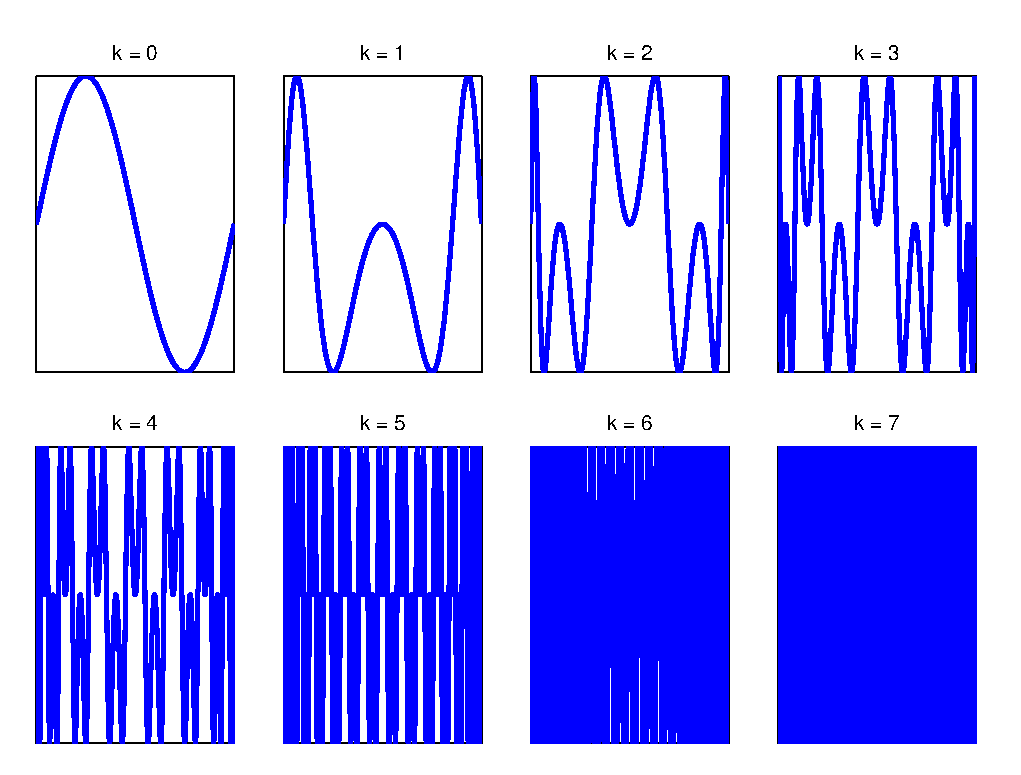
\includegraphics[width=0.7\textwidth,trim=1cm 1cm 0cm 0cm]{funcutofflogisticmap.eps}
}
%%%%%%%%%%%%%%%%%%%%%%%%%%%%%%%%%%%%%%%%%%%%%%%%%%%%%%%%%%%%%%%%%%%%%%%%%%
\newpage
\oursection{Markov Chain Model}
\begin{tabular}{rl}%\setlength{\tabcolsep}{-30mm}
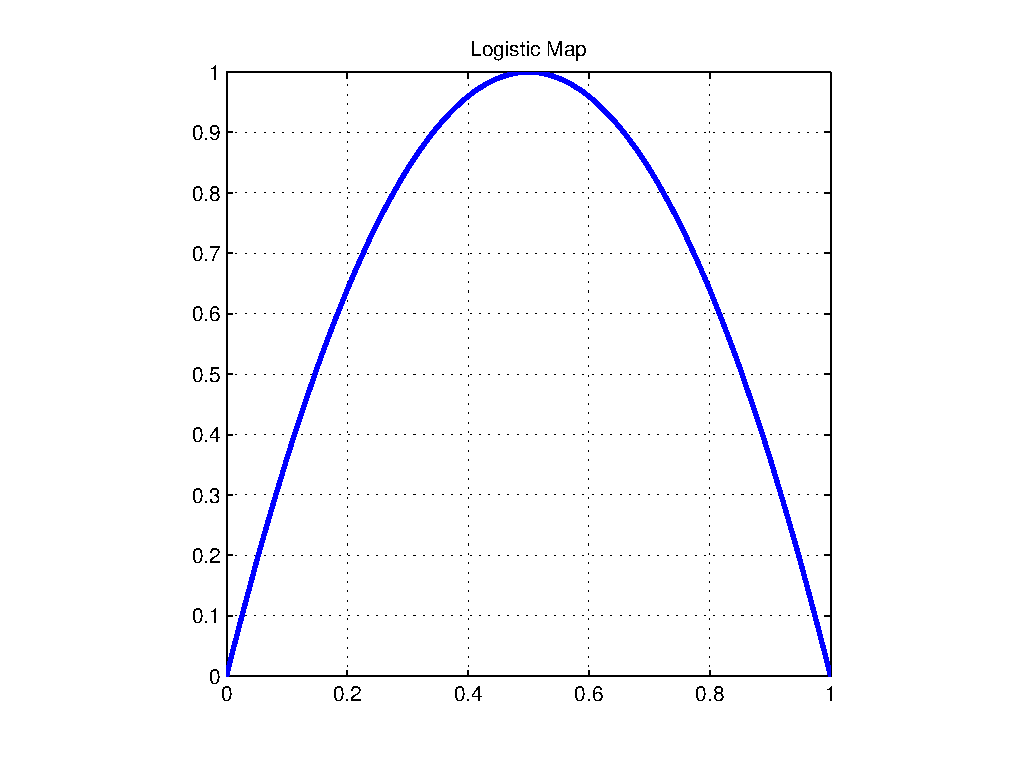
\includegraphics[width=0.44\textwidth,trim=1cm 1cm 0cm 0cm]{logisticmap}&
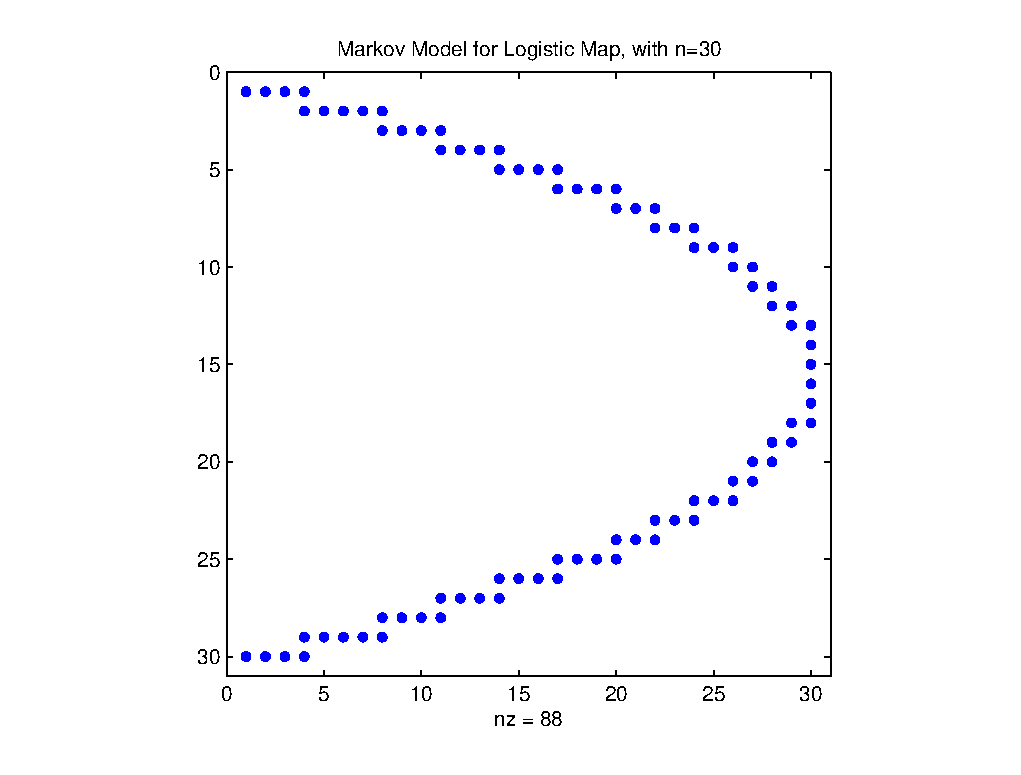
\includegraphics[width=0.44\textwidth,trim=1cm 1cm 0cm 0cm]{logisticmapA}
\end{tabular}
\begin{itemize}
\setlength{\parskip}{0pt}  \setlength{\itemsep}{5pt} \setlength{\topsep}{0pt}
 \item $\lim_{n \rightarrow \infty} A_n^T = A^T $, $(P_S)$, and $\lim_{n \rightarrow \infty}A_n = A $, $(U_S)$
 \item Extremely sparse, easy to evolve the system, parallelizable.
 \item Creates some error, propotional to the grid size.
 \item Consider the error generated by the approximation to be diffusion.
\end{itemize}

%%%%%%%%%%%%%%%%%%%%%%%%%%%%%%%%%%%%%%%%%%%%%%%%%%%%%%%%%%%%%%%%%%%%%%%%%%
\newpage
\oursection{Logistic Map with Diffusion}
\begin{tabular}{rl}%\setlength{\tabcolsep}{-30mm}
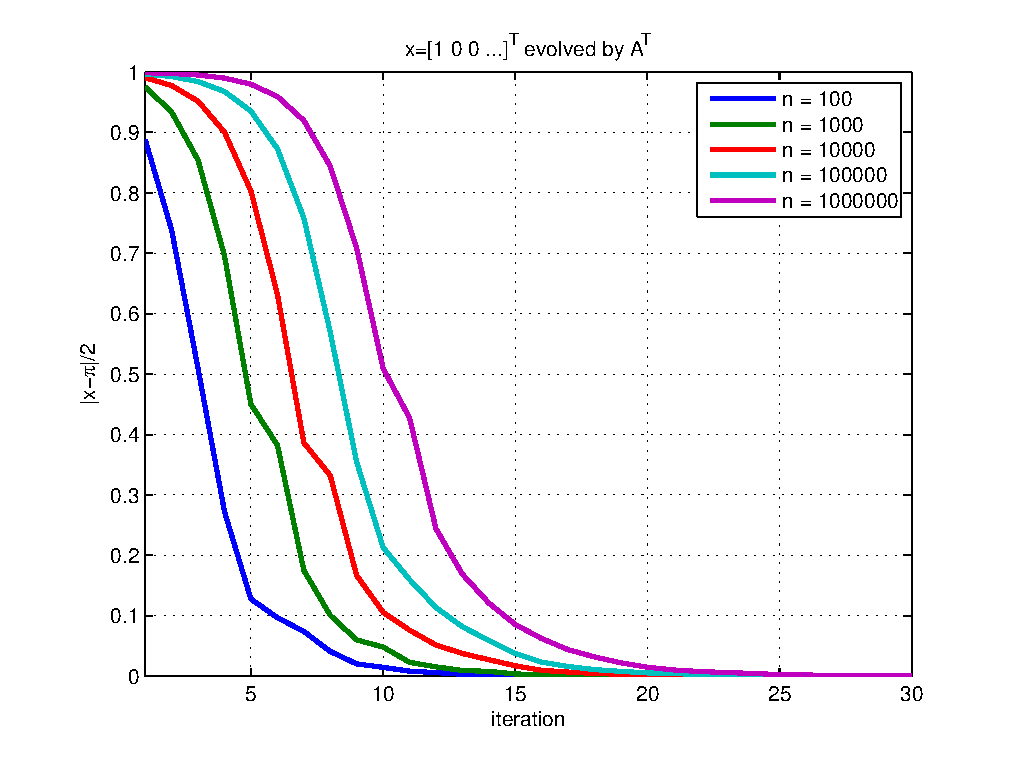
\includegraphics[width=0.44\textwidth,trim=1cm 1cm 0cm 0cm]{logisticxcutoff}&
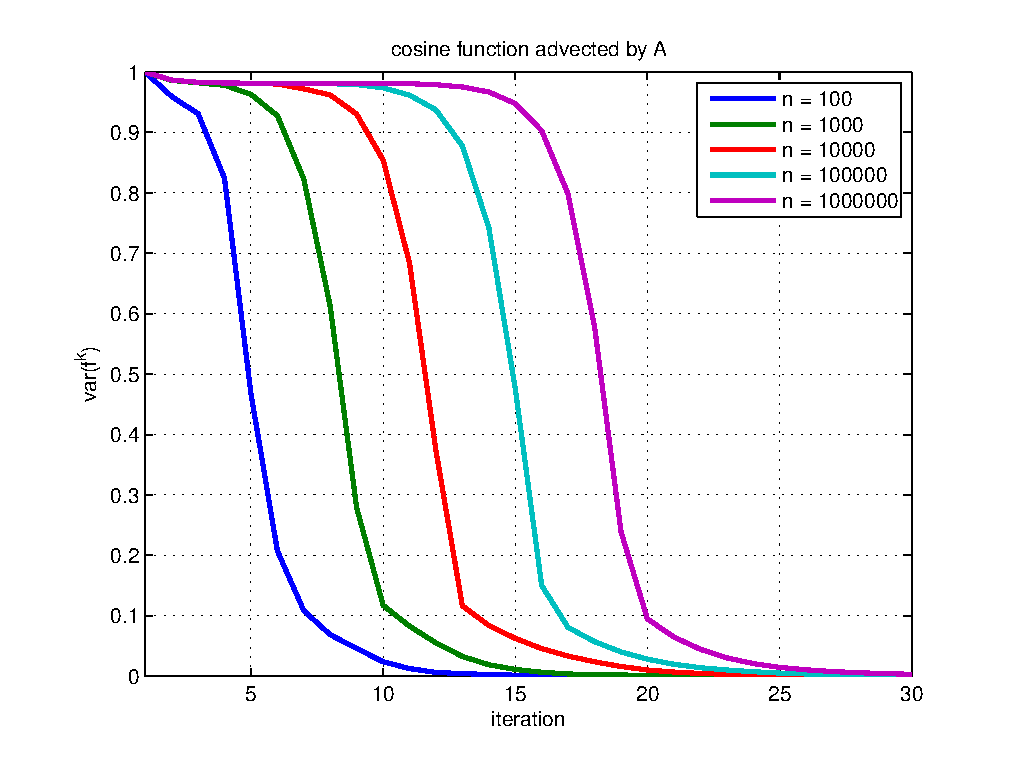
\includegraphics[width=0.44\textwidth,trim=1cm 1cm 0cm 0cm]{logisticfcutoff}
\end{tabular}
\begin{itemize}
\setlength{\parskip}{0pt}  \setlength{\itemsep}{3pt} \setlength{\topsep}{0pt}
 \item $n$:number of grids in discretization
 \item Left: $\omega^{k+1} = A_n^T \omega^{k}$, $\omega^0 = [1,0,..,0]\in \mathbb{R}^n$
 \item Right: $f^{k+1} = A_n f^{k}$, $f^{0} = g_n(\cos(2\pi x))\in \mathbb{R}^n$
 \item Cutoffs are observed both in simulations of $A$ and $A^T$. 
\end{itemize}

%%%%%%%%%%%%%%%%%%%%%%%%%%%%%%%%%%%%%%%%%%%%%%%%%%%%%%%%%%%%%%%%%%%%%%%%%
\newpage

\includegraphics[width=1\textwidth,trim=1cm 1cm 0cm 11cm]{Standardmapexample}

\textbf{Standard Map}
  \begin{eqnarray*}
               x_1' &=&  x_1+x_2 +\epsilon \sin{2 \pi x_1} (\mbox{ mod } 1)\\
               x_2' &=&  x_2 +\epsilon \sin{2 \pi x_1}     (\mbox{ mod } 1)
  \end{eqnarray*}

%%%%%%%%%%%%%%%%%%%%%%%%%%%%%%%%%%%%%%%%%%%%%%%%%%%%%%%%%%%%%%%%%%%%%%%%
\newpage
\centerline{
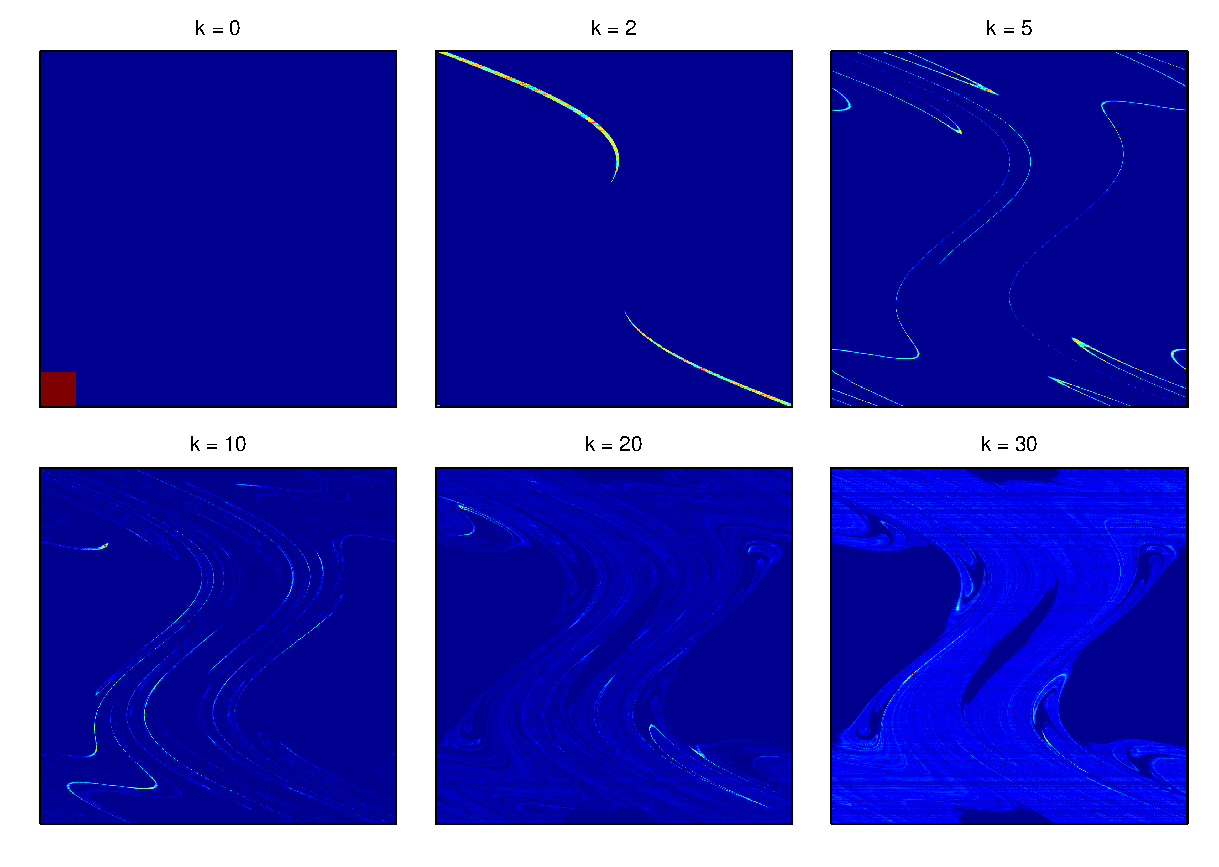
\includegraphics[width=0.7\textwidth,trim=1cm 1cm 1cm 1cm]{demostandardmapsing.eps}
}
\begin{itemize}
\setlength{\topsep}{0cm}\setlength{\parskip}{0cm}\setlength{\parsep}{0cm}\setlength{\itemsep}{0cm}
\item $\omega^{k+1} = A_n^T \omega^{k}$, with $\omega^0$ unifromly concentrated in a square in the lower-left corner 
%\item Zoom in on the first figure to see the initial distribution (upper-left corner).
\end{itemize}

%%%%%%%%%%%%%%%%%%%%%%%%%%%%%%%%%%%%%%%%%%%%%%%%%%%%%%%%%%%%%%%%%%%%%%%%
\newpage
\centerline{
\includegraphics[width=0.7\textwidth,trim=1cm 1cm 1cm 1cm]{demostandardmapcos.eps}
}
\begin{itemize}
\setlength{\topsep}{0cm}\setlength{\parskip}{0cm}\setlength{\parsep}{0cm}\setlength{\itemsep}{0cm}
\item $f^{k+1} = A_n f^{k}$, $ f^0 = g_n(\cos(2\pi x_2))$
\end{itemize}

%%%%%%%%%%%%%%%%%%%%%%%%%%%%%%%%%%%%%%%%%%%%%%%%%%%%%%%%%%%%%%%%%%%%%%%%%
\newpage
\centerline{
\begin{tabular}{rl}
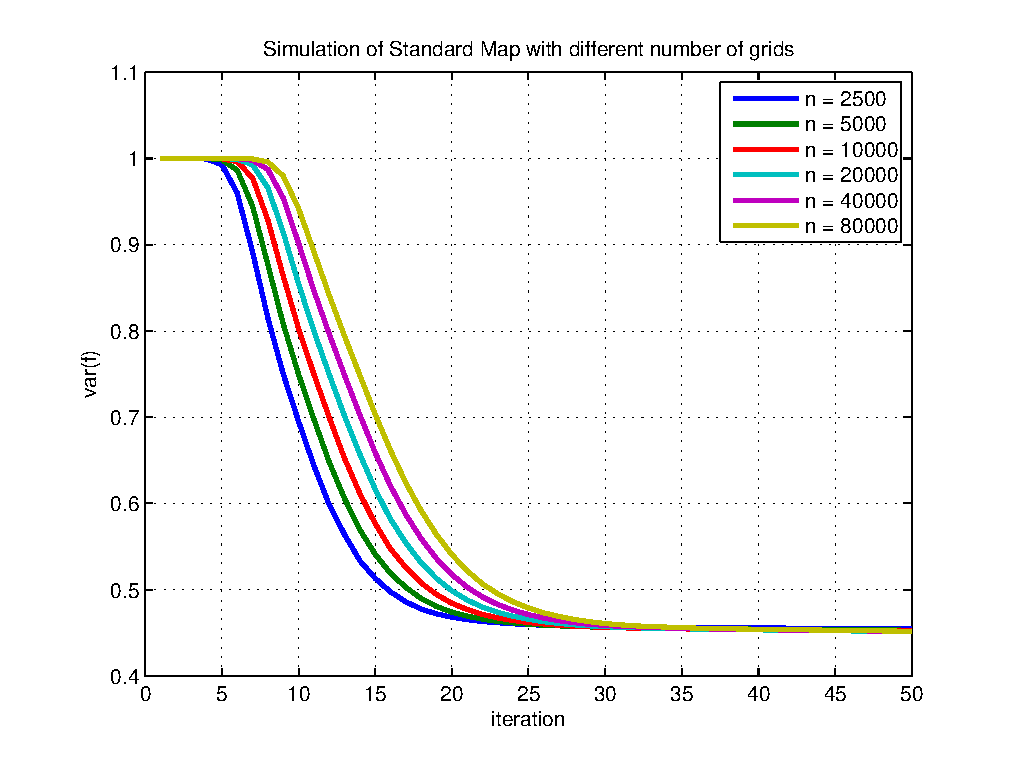
\includegraphics[width=0.35\textwidth,trim=1cm 1cm 0cm 0cm]{standardmapcutoff}&
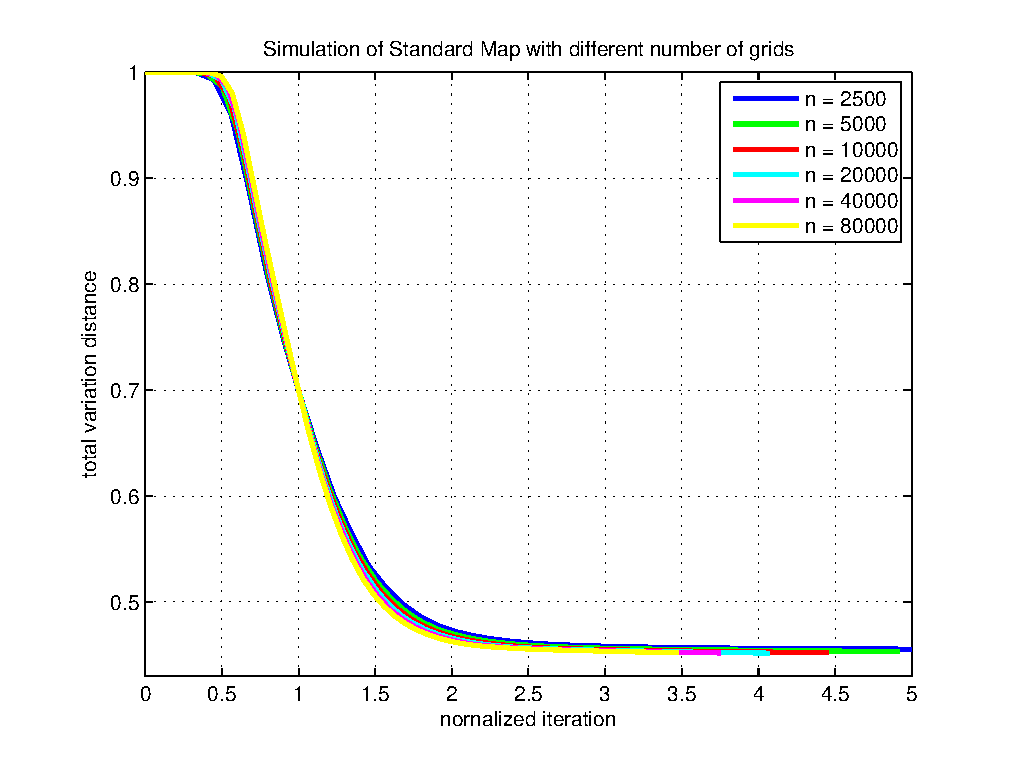
\includegraphics[width=0.35\textwidth,trim=1cm 1cm 0cm 0cm]{standardmapcutoffn}
\end{tabular}
}
\centerline{
\begin{tabular}{rl}
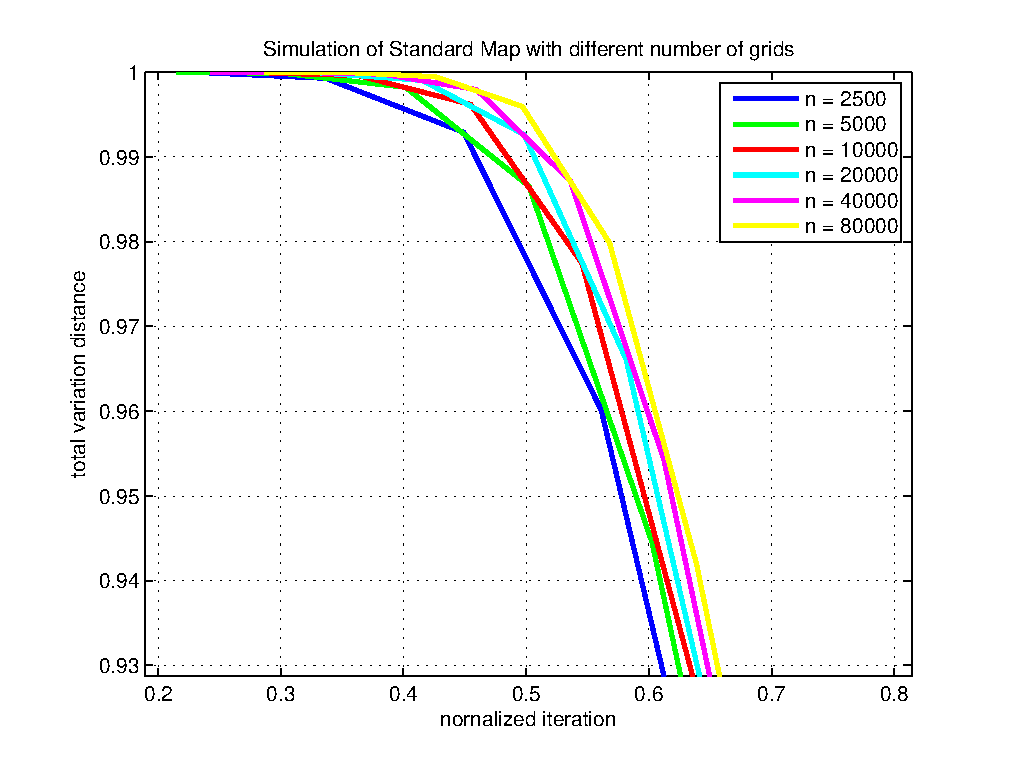
\includegraphics[width=0.35\textwidth,trim=1cm 1cm 0cm 0cm]{standardmapcutoffmacro}
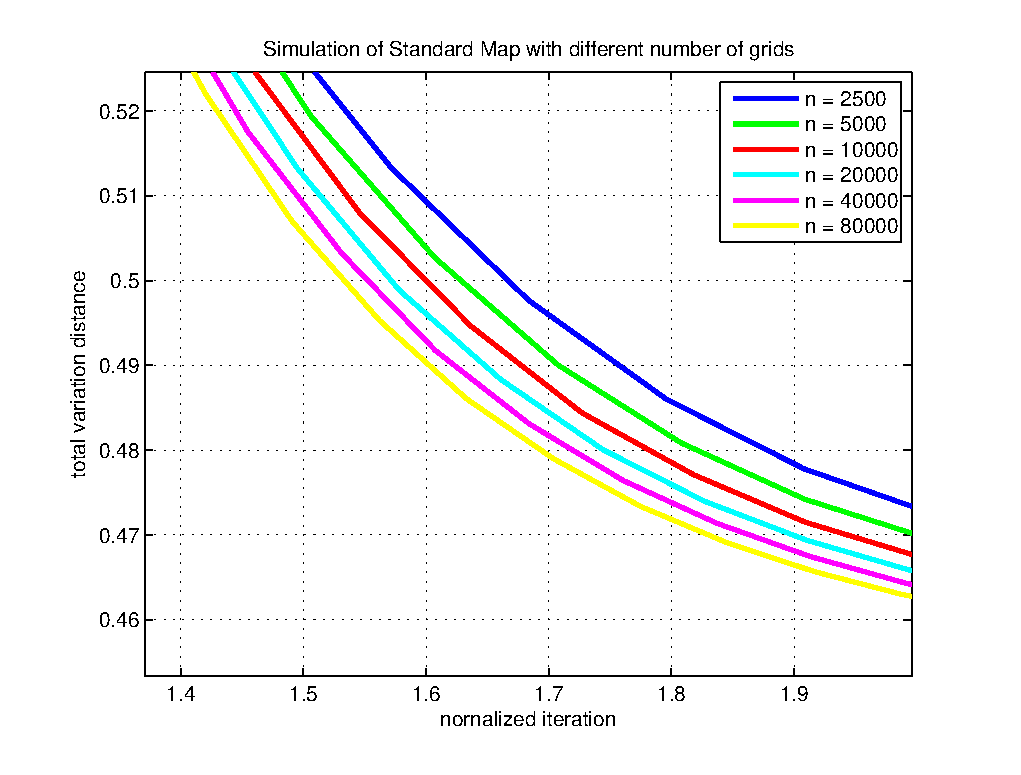
\includegraphics[width=0.35\textwidth,trim=1cm 1cm 0cm 0cm]{standardmapcutoffmacro2}
\end{tabular}
}
Number of states: $6.4G$. Extremely hard to prove cutoff even numerically!

%%%%%%%%%%%%%%%%%%%%%%%%%%%%%%%%%%%%%%%%%%%%%%%%%%%%%%%%%%%%%%%%%%%%%%%%%
\newpage
\oursection{Conclusion}
\begin{itemize}
\item Cutoff happens very often in the simulation of chaotic map with small diffusion.
\item Phase change exists in both chaotic mixing and chaotic randomizing.
\item Define a quantitative measure of chaos through cutoff?
\end{itemize}


%%%%%%%%%%%%%%%%%%%%%%%%%%%%%%%%%%%%%%%%%%%%%%%%%%%%%%%%%%%%%%%%%%%%%%%%%
%\newpage

%\begin{figure}
% \centerline{
%  \scalebox{0.5}[0.5]{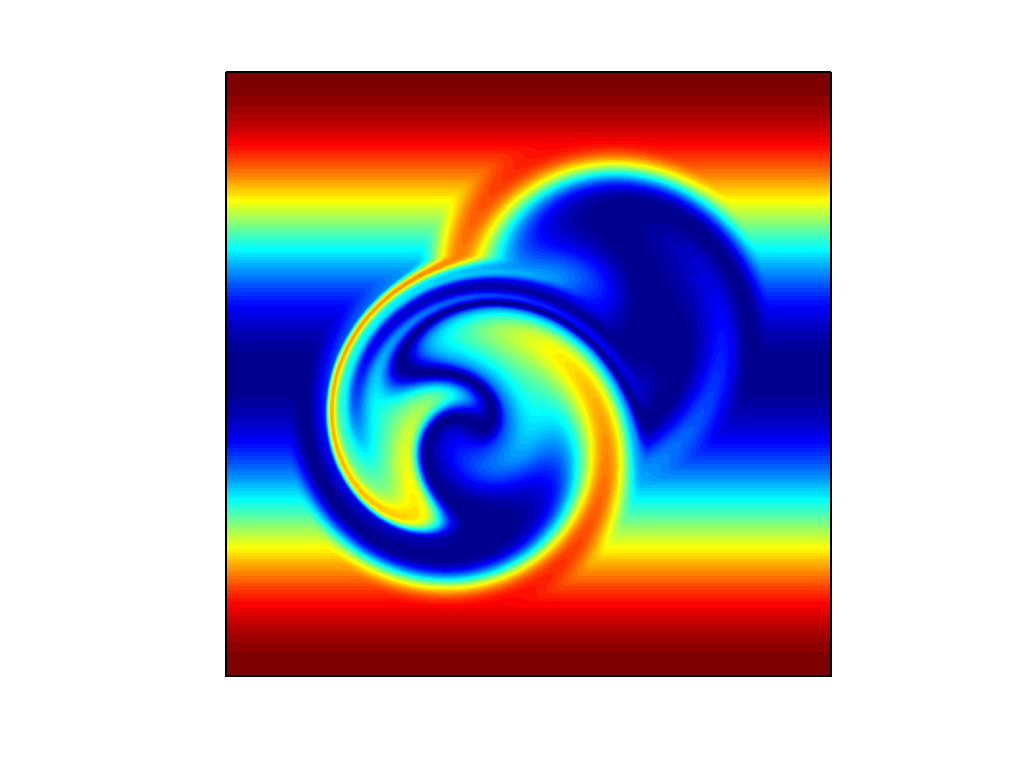
\includegraphics{ltmiter20.eps}}
%  \scalebox{0.5}[0.5]{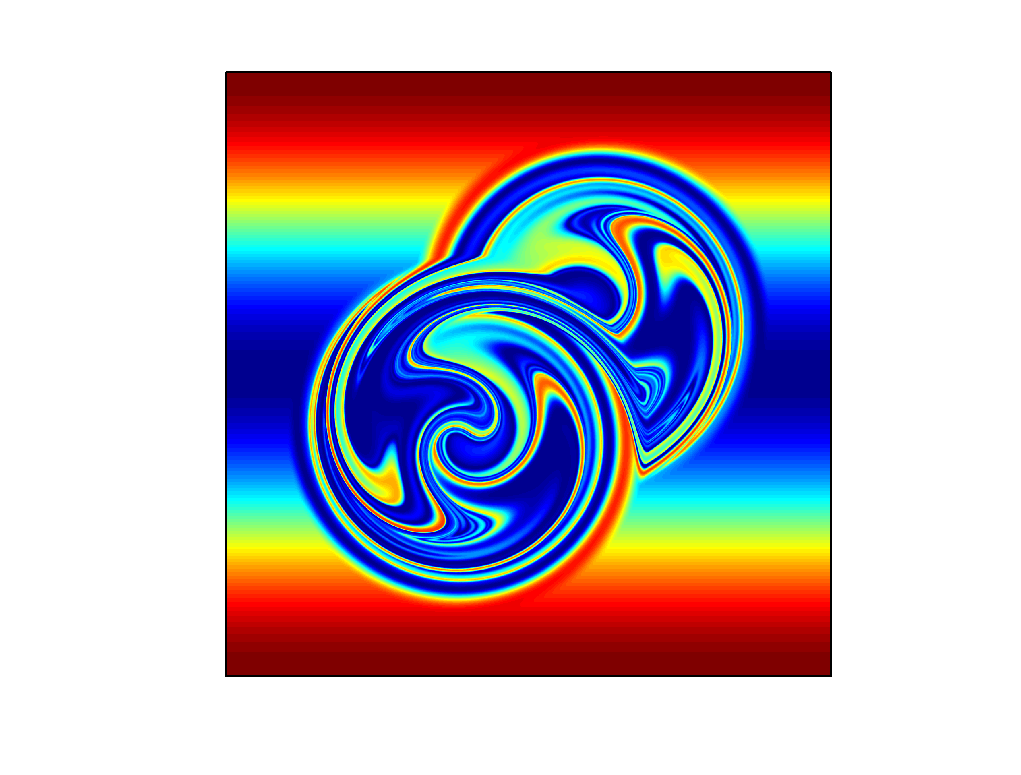
\includegraphics{ltmiter60.eps}}
%  }
%  \centerline{
%  \scalebox{0.5}[0.5]{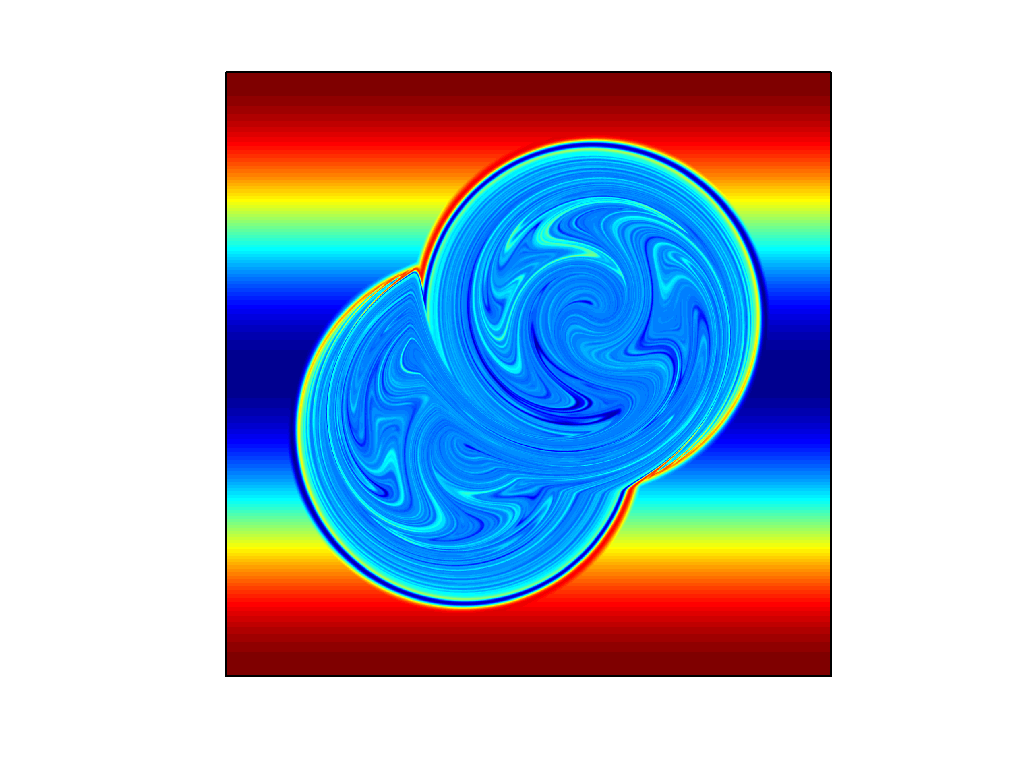
\includegraphics{ltmiter250.eps}}
%  \scalebox{0.5}[0.5]{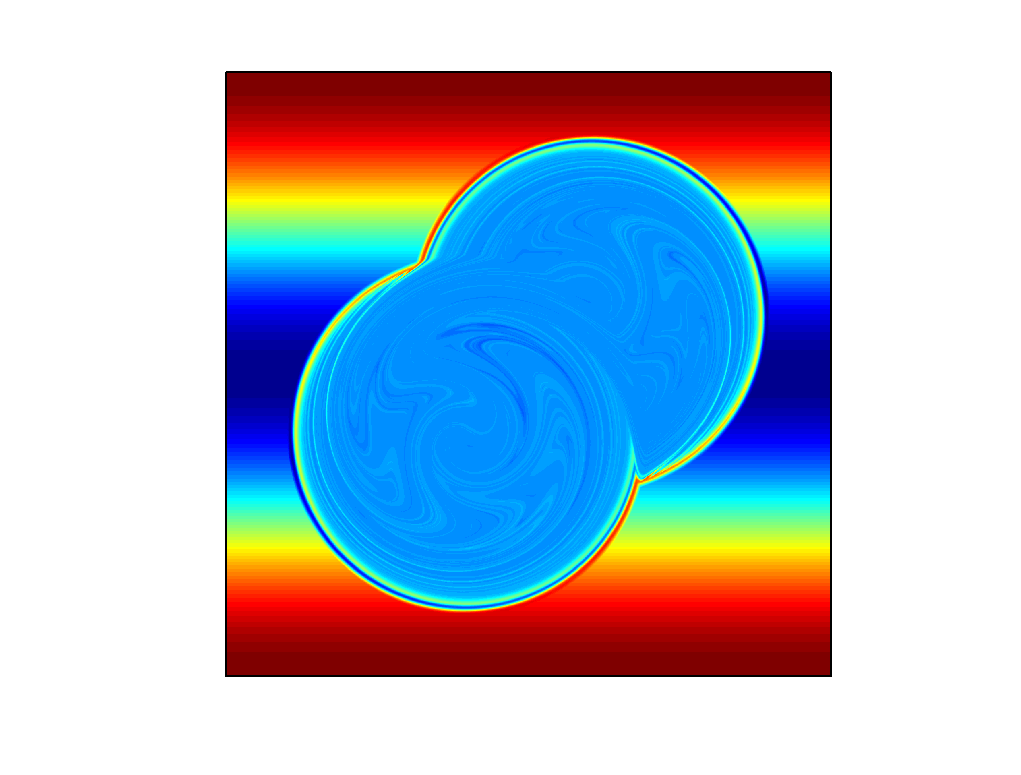
\includegraphics{ltmiter500.eps}}
%  }
%  \caption{LTM simulations with initial condition $c(x,y)=\cos(y)$,
%          (a)iter=20, (b)iter=40, (c)iter=250, (d)=iter=500}
%  \label{ltmiter}
%\end{figure}



%%%%%%%%%%%%%%%%%%%%%%%%%%%%%%%%%%%%%%%%%%%%%%%%%%%%%%%%%%%%%%%%%%%%%%%%%
%\newpage
%\oursection{Mixing Channel}
%\begin{itemize}
%\item A tube with some internal structure to stir the flow.
%\item Think the mixing channel as a map $S$. The liquid to be mixed is a set of small particles with different colors.
%\item Connect many of this channel together to achive successive mapping. Periodical boundry condition.
%\item The flow is stationary so the velocity profile in the inlet and outlet are not functions of time.  
%\item the velocity profile means the number of particles go in (and out) the channel per unit time at point $x$.
%\end{itemize}



%%%%%%%%%%%%%%%%%%%%%%%%%%%%%%%%%%%%%%%%%%%%%%%%%%%%%%%%%%%%%%%%%%%%%%%%%
%\newpage
%\begin{itemize}
%\item Consider there are white and black particles. 
%$$color(x) \equiv \frac{\text{number of black particles at }x}{\text{number of total particles at }x} \in [0,1]$$
%\item Question: How is the color evolved by the mixing channel?
%\item 
%\item   
%\end{itemize}





%%%%%%%%%%%%%%%%%%%%%%%%%%%%%%%%%%%%%%%%%%%%%%%%%%%%%%%%%%%%%%%%%%%%%%%%%%
\end{document}
